\documentclass[11pt,a4paper]{article}

\usepackage{fontspec}
\usepackage[margin=21mm]{geometry}
\usepackage{amsmath,amssymb}
\usepackage{booktabs,longtable,array,tabularx}
\usepackage{graphicx}
\usepackage{caption}
\usepackage{subcaption}
\usepackage{xcolor}
\usepackage{hyperref}
\usepackage{enumitem}
\usepackage{float}

\defaultfontfeatures{Ligatures=TeX,Scale=MatchLowercase}
\IfFontExistsTF{Noto Sans CJK KR}{
  \setmainfont{Noto Sans CJK KR}[
    ItalicFeatures={FakeSlant=0.18},
    BoldItalicFeatures={FakeSlant=0.18}
  ]
  \setsansfont{Noto Sans CJK KR}[
    ItalicFeatures={FakeSlant=0.18},
    BoldItalicFeatures={FakeSlant=0.18}
  ]
}{
  \IfFontExistsTF{Apple SD Gothic Neo}{
    \setmainfont{Apple SD Gothic Neo}[
      ItalicFeatures={FakeSlant=0.18},
      BoldItalicFeatures={FakeSlant=0.18}
    ]
    \setsansfont{Apple SD Gothic Neo}[
      ItalicFeatures={FakeSlant=0.18},
      BoldItalicFeatures={FakeSlant=0.18}
    ]
  }{
    \setmainfont{NanumGothic}[
      ItalicFeatures={FakeSlant=0.18},
      BoldItalicFeatures={FakeSlant=0.18}
    ]
    \setsansfont{NanumGothic}[
      ItalicFeatures={FakeSlant=0.18},
      BoldItalicFeatures={FakeSlant=0.18}
    ]
  }
}
\IfFontExistsTF{DejaVu Sans Mono}{
  \setmonofont{DejaVu Sans Mono}
}{
  \IfFontExistsTF{Menlo}{
    \setmonofont{Menlo}
  }{
    \setmonofont{Liberation Mono}
  }
}
\XeTeXlinebreaklocale "ko"
\XeTeXlinebreakskip = 0pt plus 1pt

\hypersetup{
  colorlinks=true,
  linkcolor=blue!50!black,
  urlcolor=blue!50!black,
  citecolor=blue!50!black,
  pdftitle={UUV MuJoCo v2.2 current-focus technical report},
  pdfauthor={OpenAI Codex}
}

\setlength{\parskip}{0.52em}
\setlength{\parindent}{0pt}
\setlength{\emergencystretch}{3em}
\renewcommand{\arraystretch}{1.22}
\newcolumntype{Y}{>{\raggedright\arraybackslash}X}
\newcommand{\code}[1]{\nolinkurl{#1}}
\captionsetup{
  font=small,
  labelfont=bf,
  justification=raggedright,
  singlelinecheck=false,
  skip=6pt
}

\title{UUV MuJoCo v2.2 current 모델 중심 기술 보고서\\
\large docsource 최신 actual 데이터와 현재 repository 설정을 함께 반영한 재정리본}
\author{}
\date{2026-04-06}

\begin{document}
\maketitle
\tableofcontents
\clearpage

\section{문서 범위와 데이터 기준}

이번 문서는 \textbf{legacy를 길게 비교하는 보고서가 아니라, current 모델을 해설하는 문서}로 다시 정리했다. 따라서 legacy는 구조적 차이만 짧게 적고, 본문 대부분은 current runtime의 물리엔진 분해, thrust path, buoyancy model 비교, latest actual reference에 집중한다.

직접 사용한 입력은 아래와 같다.

\begin{itemize}[leftmargin=2em]
  \item \code{document/docsource/uuv_v22_latest_report_metrics.json}
  \item \code{document/docsource/uuv_v22_current_focus_metrics.json}
  \item \code{document/docsource/measurement_current_mode_path_latest_v30.json}
  \item \code{document/docsource/measurement_summary_current_heavefix_latest_v30.json}
  \item \code{uuv_mujoco/v2.2/config/sim_profiles.json}
  \item \code{uuv_mujoco/v2.2/config/thruster_params.json}
\end{itemize}

여기서 숫자는 두 그룹으로 구분했다.

\begin{enumerate}[leftmargin=2em]
  \item \textbf{latest actual reference}: 2026-04-06 rosbag에서 뽑은 current mode-path / step summary
  \item \textbf{current repository snapshot}: 보고서 생성 시점의 \code{sim\_profiles.json}, \code{thruster\_params.json}, \code{tank\_current\_scene.xml}
\end{enumerate}

\section{한 장 요약}

\begin{itemize}[leftmargin=2em]
  \item current v2.2는 \textbf{MuJoCo built-in ellipsoid fluid} 와 \textbf{Python custom thrust / hydrostatics} 를 결합한 하이브리드 구조다.
  \item legacy 대비 current latest actual 평균값은 trajectory path 73.65\%, horizontal distance 93.90\%, max pitch 99.57\%, max roll 71.72\% 감소다. 여기서는 이 숫자를 결과 컨텍스트로만 사용하고, 본문 분석은 current에 집중한다.
  \item current snapshot의 핵심 값은 \code{thruster\_force\_max} = 32\,N, \code{vertical\_thruster\_gain\_scale} = 1.45, \code{yaw\_torque\_scale} = 1.5, \code{buoyancy\_scale} = 1.008, \code{cob\_torque\_scale} = 1 다.
  \item thrust path는 \textbf{simple polynomial thruster model} 이고, shaping 파라미터는 \code{deadzone} = 0.002, \code{tau\_up} = 0.04\,s, \code{tau\_down} = 0.06\,s, \code{gain\_scale\_all} = 2.9, \code{reverse\_asymmetry} = 0.7 다.
  \item same current scene / same current thrust model / same scripted harness에서 비교하면 4-point buoyancy의 latest actual gap index는 18.72\%, single-point center 모델은 137.61\% 로 계산됐다.
\end{itemize}

\section{legacy와 current의 구조적 차이}

legacy는 이 보고서의 중심이 아니므로 구조적 차이만 남긴다.

\begin{center}
\small
\begin{tabularx}{\linewidth}{>{\raggedright\arraybackslash}p{0.26\linewidth}YY}
\toprule
항목 & legacy 구조 & current 구조 \\
\midrule
수중 유체력 주체 & custom 6-DOF hydrodynamics 중심 & MuJoCo ellipsoid fluid 중심 \\
active hydro terms & added mass, Coriolis, linear / quadratic damping 사용 & 위 항들은 기본 current 경로에서 비활성화 \\
hydrostatics & component / CoB 기반 복원토크 중심 & distributed 4-point buoyancy + restoring torque \\
thrust path & Python shaping + actuator 적용 & Python shaping + actuator 적용 \\
drag proxy scene & legacy scene / custom tuning & \code{tank\_current\_scene.xml} + ellipsoid fluid geoms \\
\bottomrule
\end{tabularx}
\end{center}

즉 current를 짧게 정의하면 \textbf{drag는 MuJoCo에 맡기고, thrust와 hydrostatics는 Python이 감싼 구조}다.

\section{current 물리엔진 블록 다이어그램}

\begin{figure}[H]
  \centering
  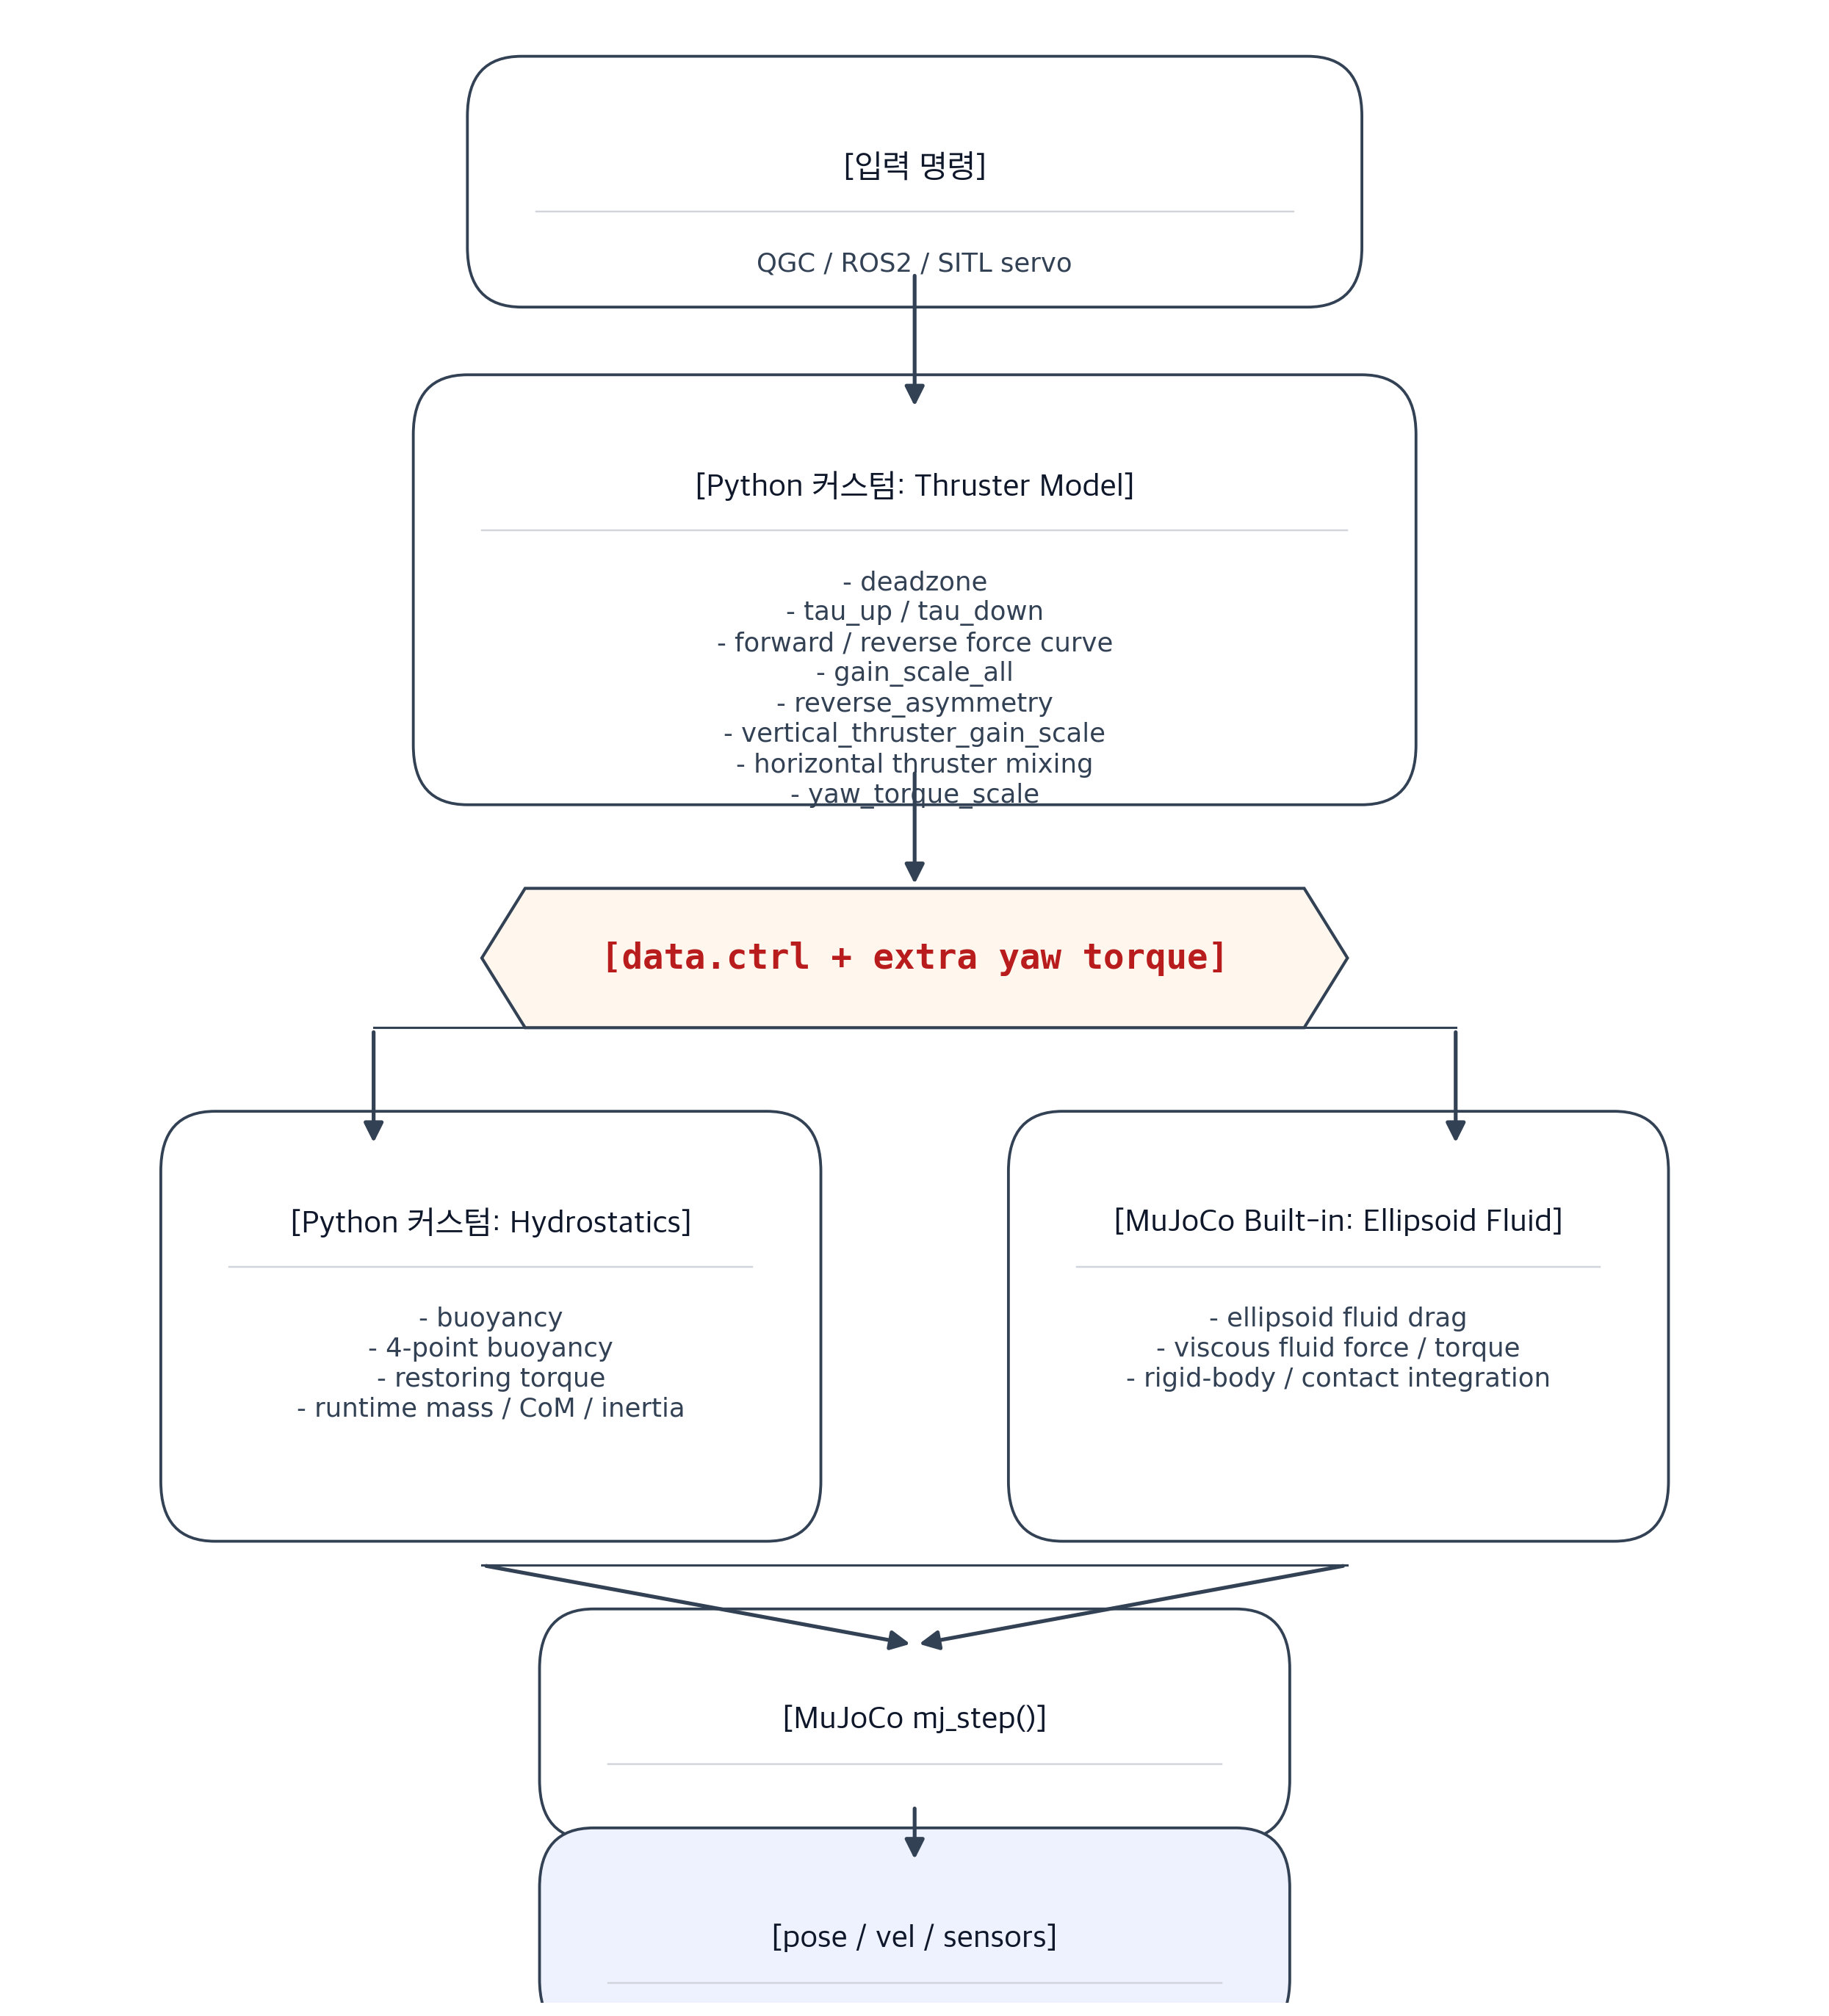
\includegraphics[width=0.88\linewidth]{figures_v22_latest/uuv_v22_latest_current_engine_block_diagram.png}
  \caption{current 모델의 물리엔진 블록 다이어그램. 입력 명령에서 thrust shaping을 거쳐 \code{data.ctrl} 와 extra yaw torque가 만들어지고, hydrostatics와 MuJoCo ellipsoid fluid가 합쳐진 뒤 \code{mj\_step()} 으로 적분된다.}
\end{figure}

\begin{center}
\small
\begin{tabularx}{\linewidth}{>{\raggedright\arraybackslash}p{0.28\linewidth}YY}
\toprule
블록 & 엔진 & current에서 실제로 하는 일 \\
\midrule
Input command & 외부 입력 & QGC / ROS2 / SITL servo가 thrust request를 만든다 \\
Python custom Thruster Model & Python & deadzone, lag, force mapping, horizontal mixing, vertical gain, extra yaw torque \\
Python custom Hydrostatics & Python & buoyancy, 4-point force distribution, restoring torque, runtime mass / CoM / inertia 재설정 \\
Ellipsoid Fluid & MuJoCo built-in & ellipsoid fluid drag, viscous fluid force / torque \\
Integration / Sensors & MuJoCo built-in & \code{mj\_step()}, rigid-body integration, 기본 센서 primitive \\
\bottomrule
\end{tabularx}
\end{center}

\begin{figure}[H]
  \centering
  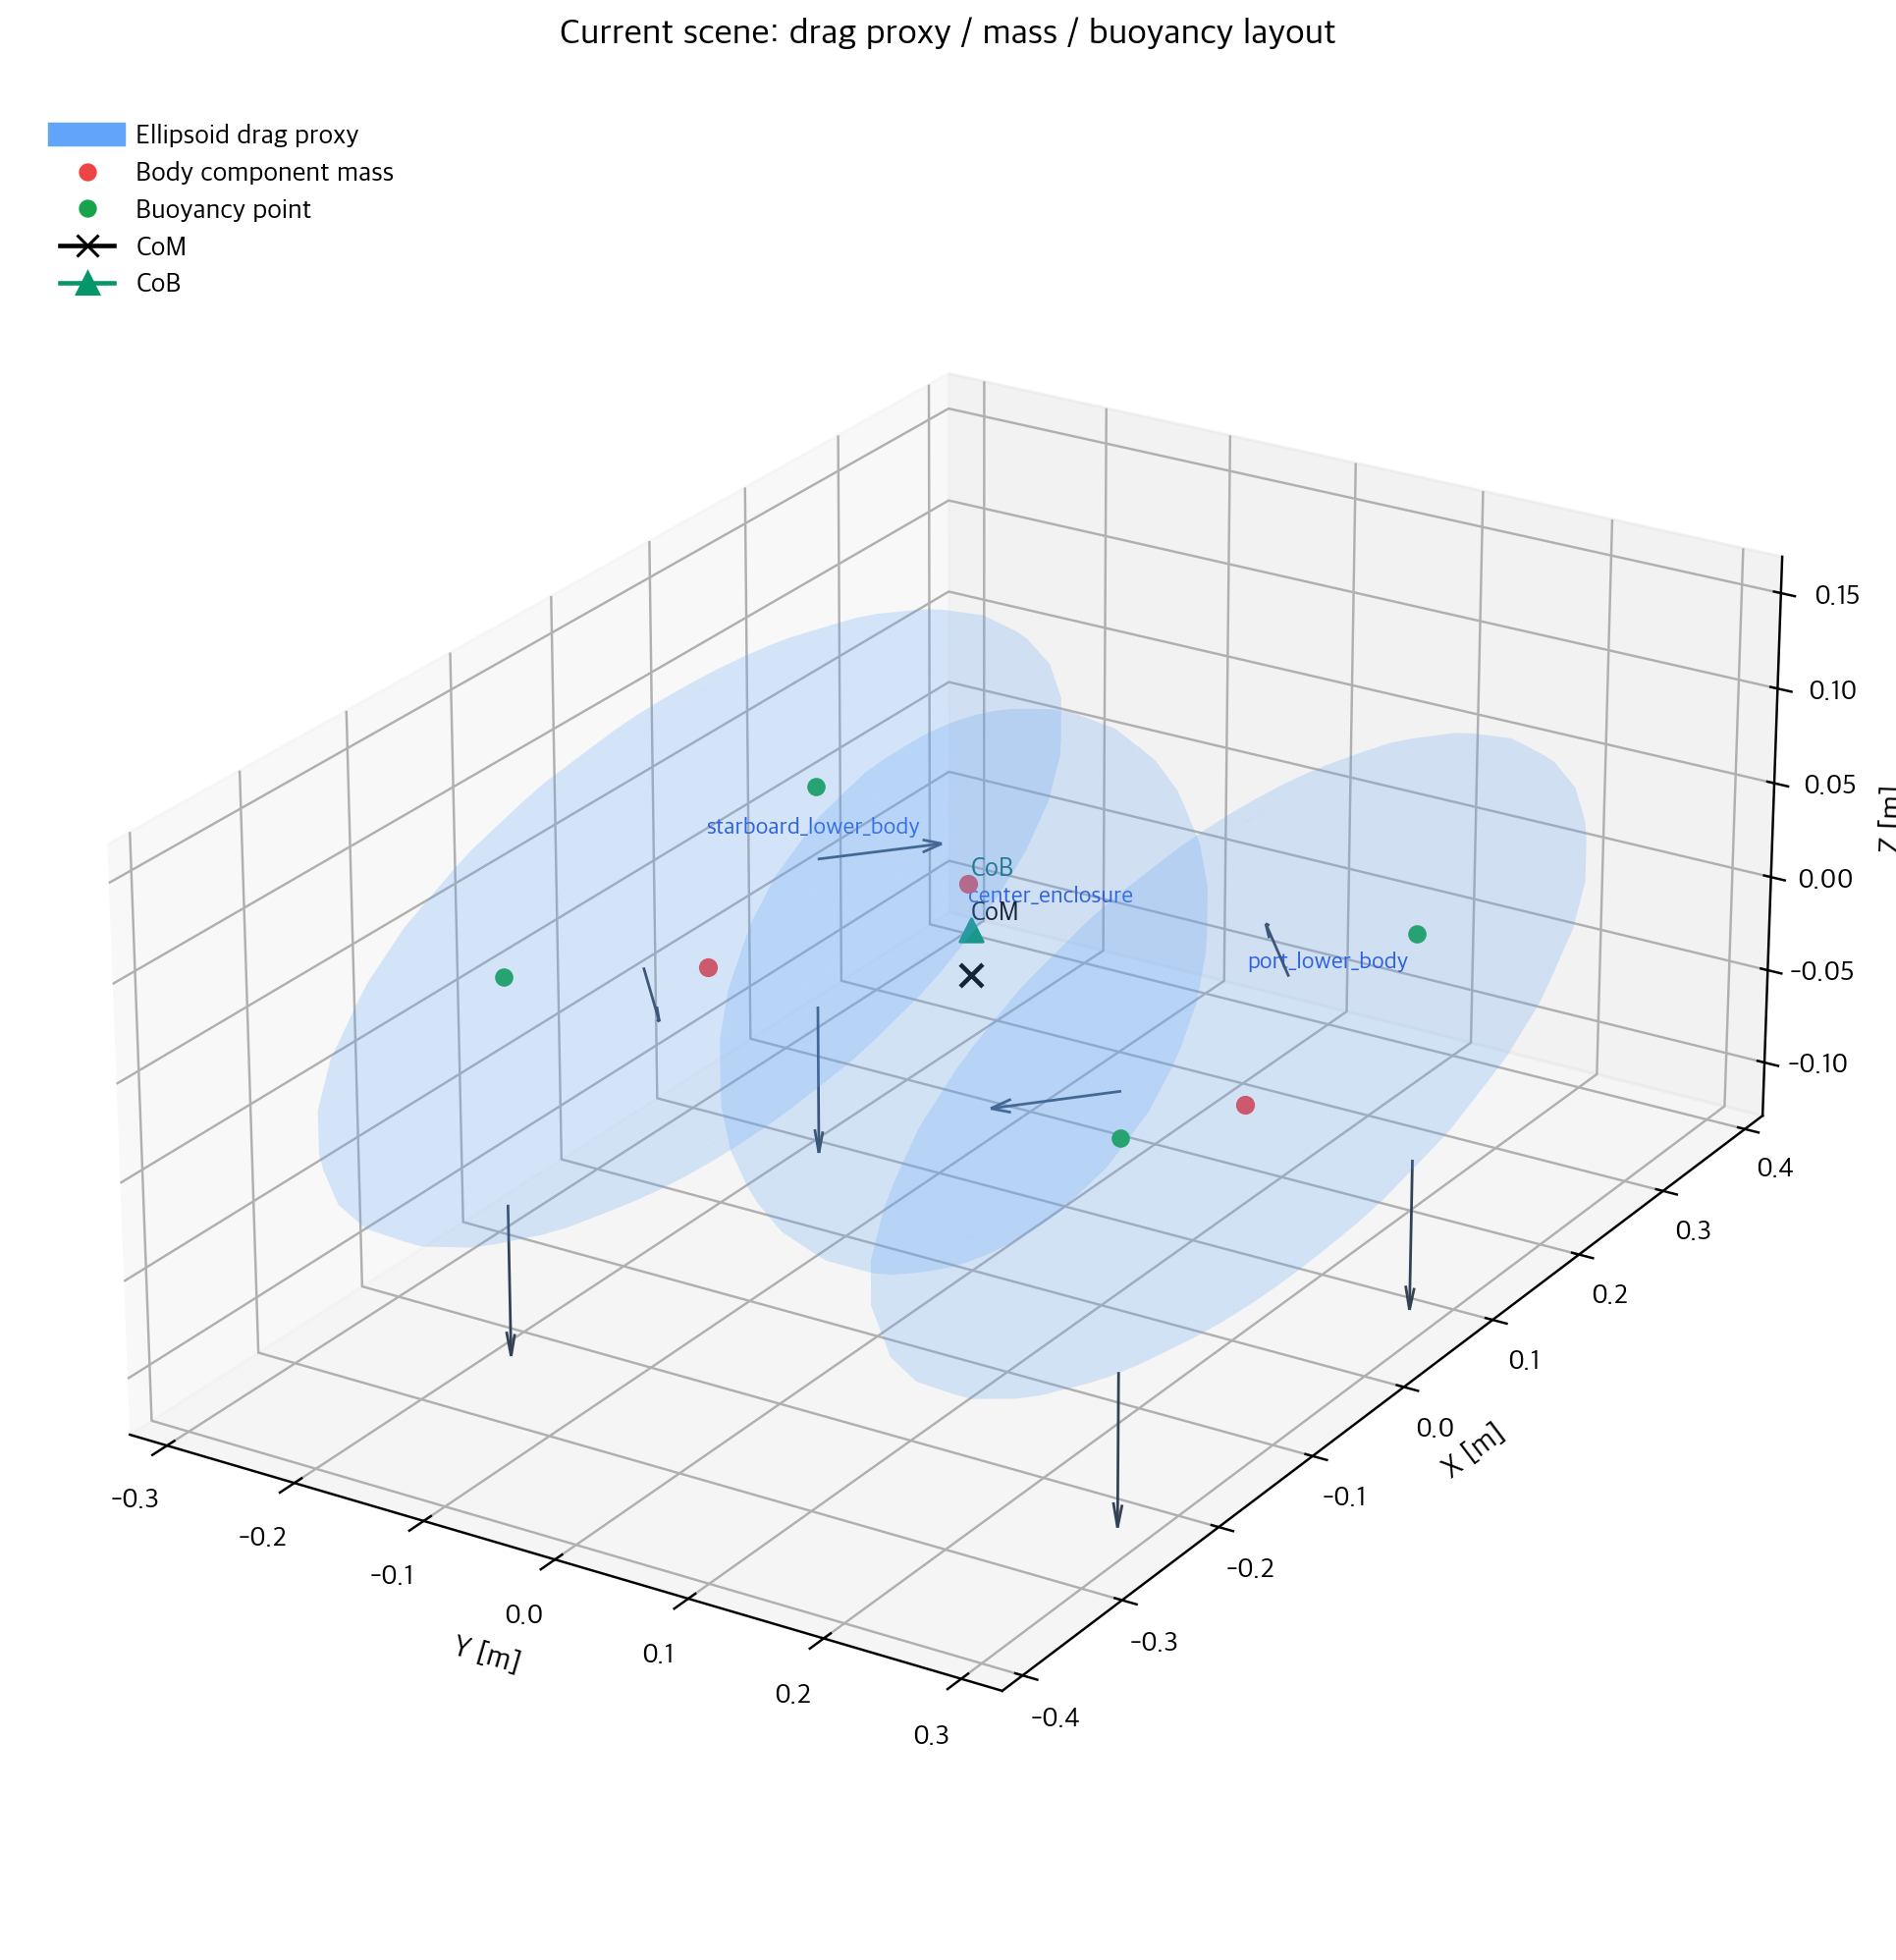
\includegraphics[width=0.88\linewidth]{figures_v22_latest/uuv_v22_latest_ellipsoid_layout.png}
  \caption{current scene의 ellipsoid drag proxy, buoyancy point, mass component, CoM, CoB 배치. current는 drag proxy와 buoyancy application point를 분리해서 쓰는 구조다.}
\end{figure}

\begin{center}
\small
\begin{tabularx}{\linewidth}{>{\raggedright\arraybackslash}p{0.30\linewidth}YY}
\toprule
항목 & current 값 & 의미 \\
\midrule
proxy total volume & 0.0426\,m$^3$ & MuJoCo ellipsoid drag 계산에 쓰이는 proxy 부피 합 \\
neutral volume & 0.0150\,m$^3$ & 15\,kg 기체의 중성부력 기준량 \\
CoM & $(-0.002, 0, 0.027)$ & runtime mass synthesis 결과 \\
CoB & $(-0.002, 0, 0.05)$ & current hydrostatics 기준 부력 중심 \\
runtime inertia & $(4.734e-07, 3.702e-07, 7.393e-07)$ & current runtime에서 실제 적용되는 관성 \\
\bottomrule
\end{tabularx}
\end{center}

\begin{center}
\small
\begin{tabularx}{\linewidth}{>{\raggedright\arraybackslash}p{0.28\linewidth}YYY}
\toprule
Geom & position [m] & semi-axis [m] & fluidcoef \\
\midrule
\code{fluid_center_enclosure} & $(-0.005, 0, 0.02)$ & $(0.205, 0.115, 0.13)$ & \shortstack[l]{0.620, 0.175,\\1.800, 0, 0} \\
\code{fluid_port_lower_body} & $(0, 0.208, 0.02)$ & $(0.37, 0.08, 0.12)$ & \shortstack[l]{0.520, 0.150,\\1.300, 0, 0} \\
\code{fluid_starboard_lower_body} & $(0, -0.208, 0.02)$ & $(0.37, 0.08, 0.12)$ & \shortstack[l]{0.520, 0.150,\\1.300, 0, 0} \\
\bottomrule
\end{tabularx}
\end{center}

\section{current thrust model}

\begin{figure}[H]
  \centering
  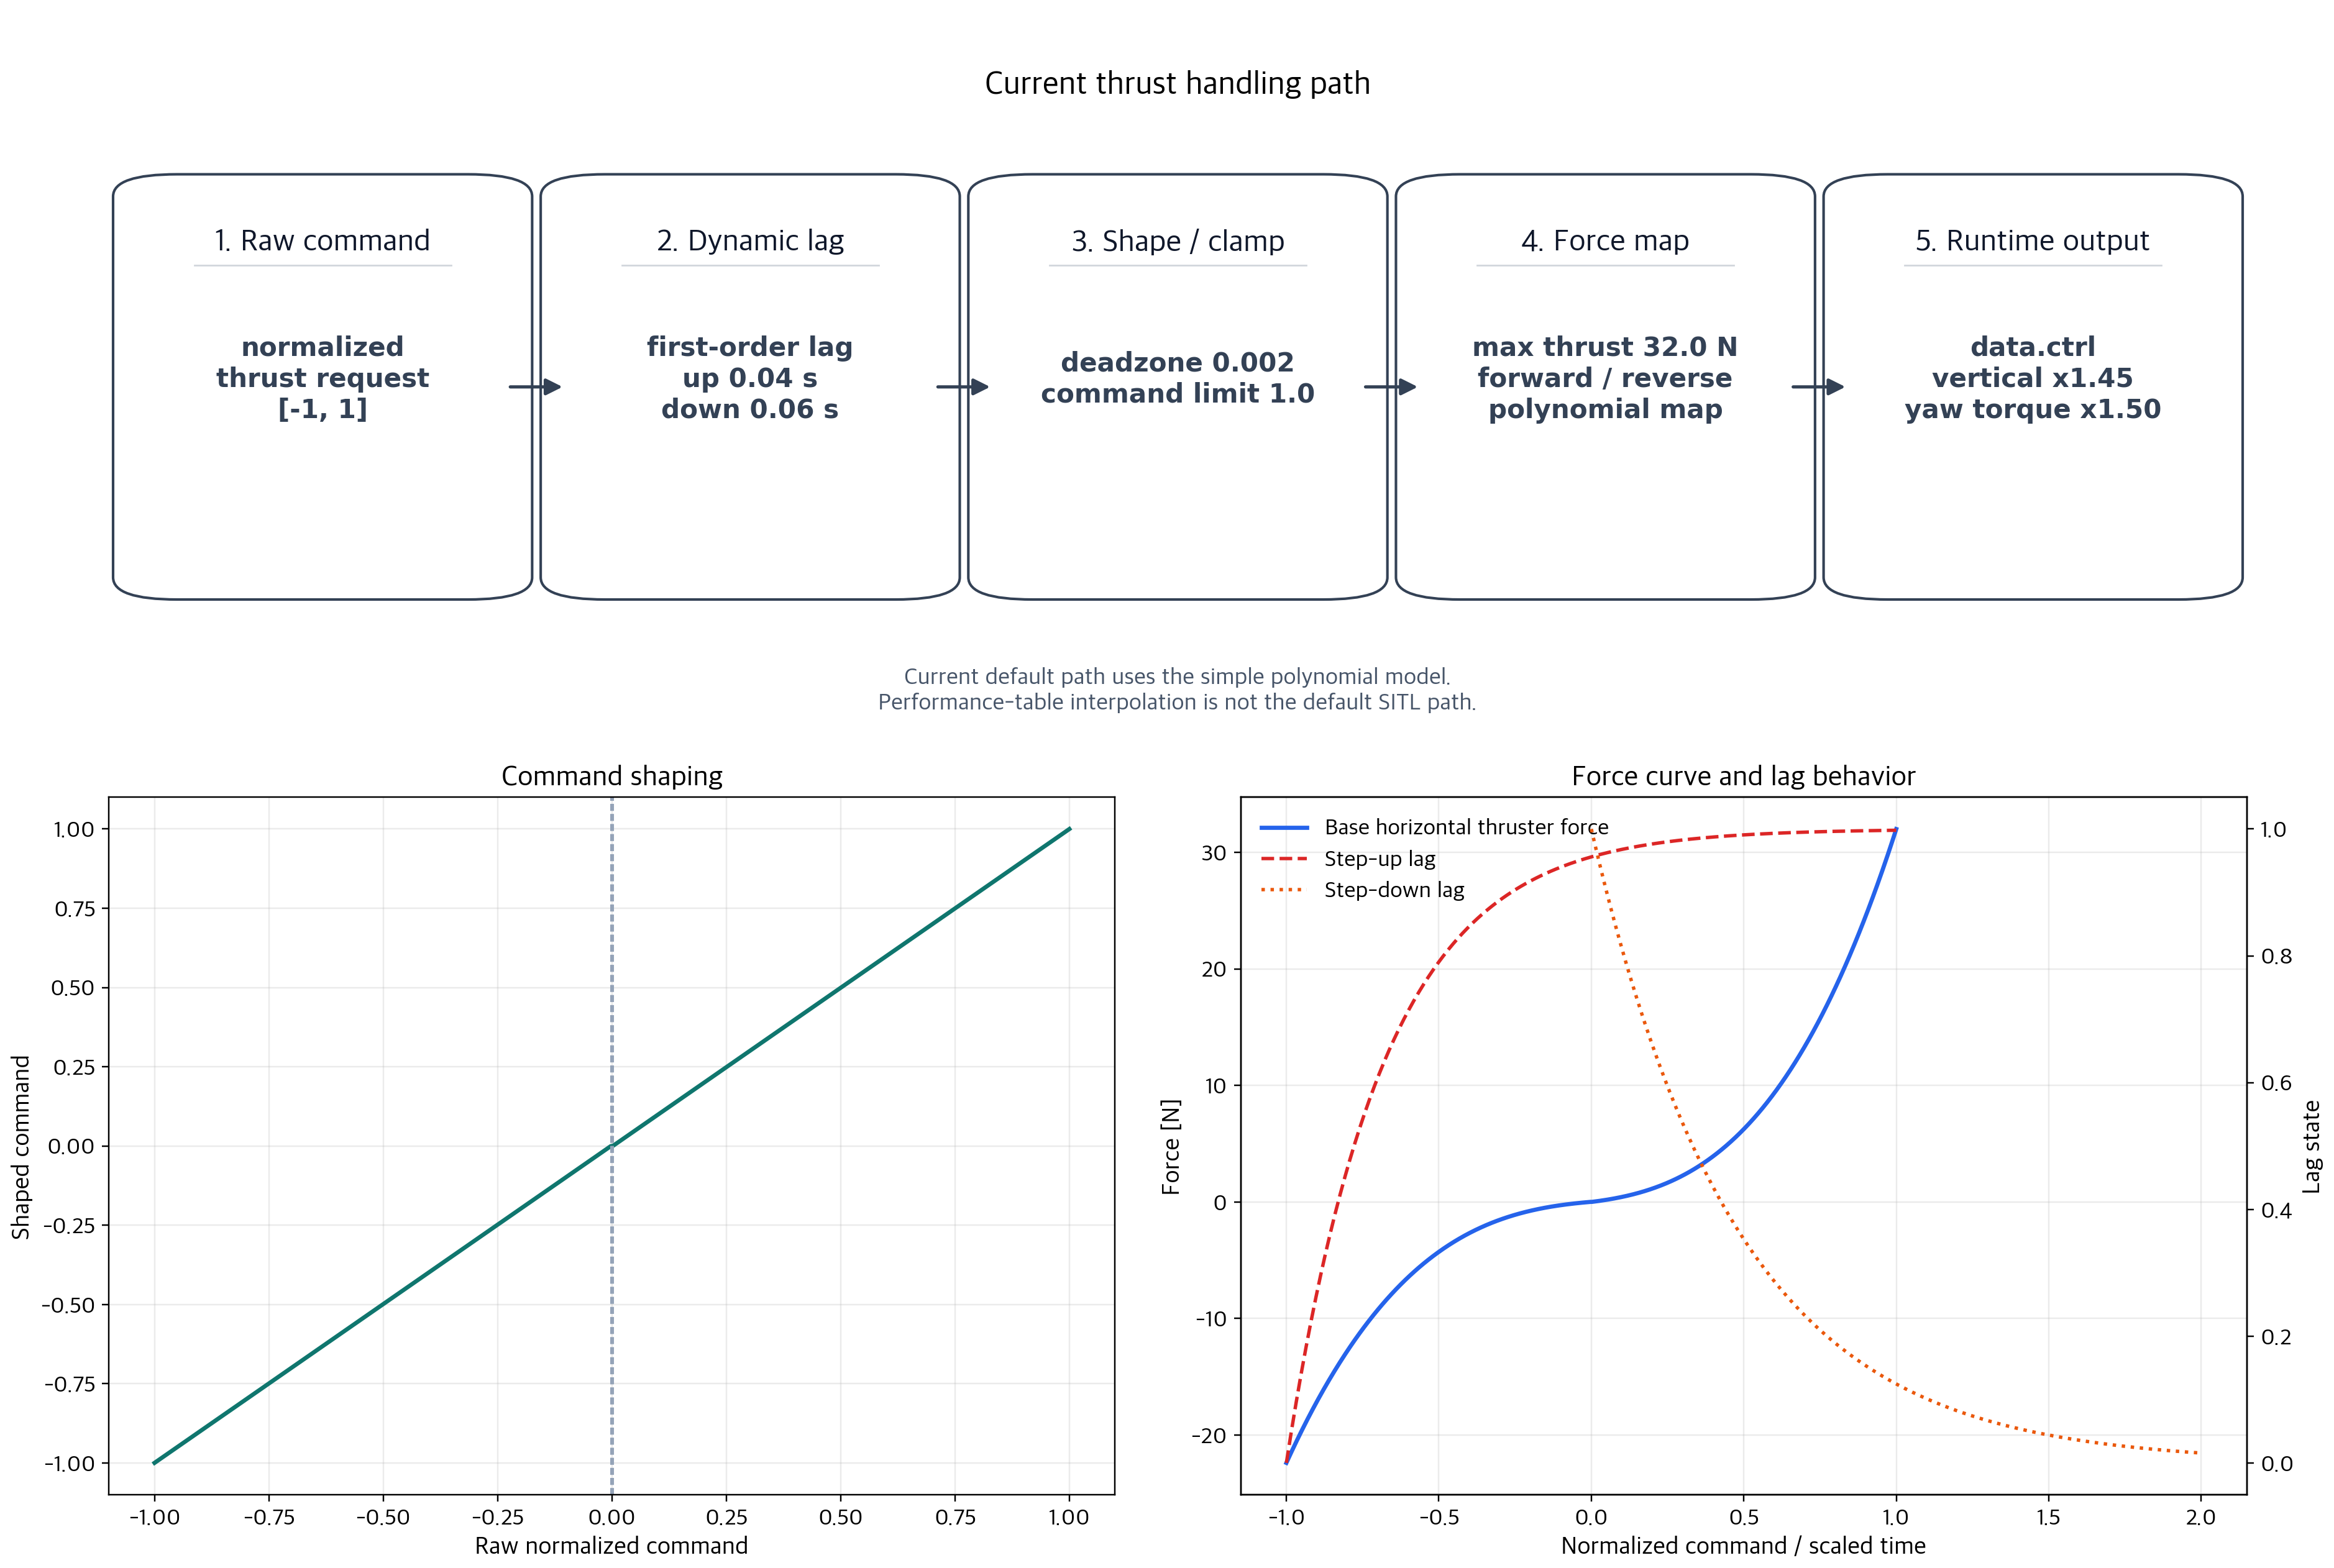
\includegraphics[width=0.98\linewidth]{figures_v22_latest/uuv_v22_latest_thruster_model_detail.png}
  \caption{current thrust path 상세. 위는 pipeline, 아래는 command shaping / force mapping / lag behavior를 current 설정값으로 그린 것이다.}
\end{figure}

\begin{figure}[H]
  \centering
  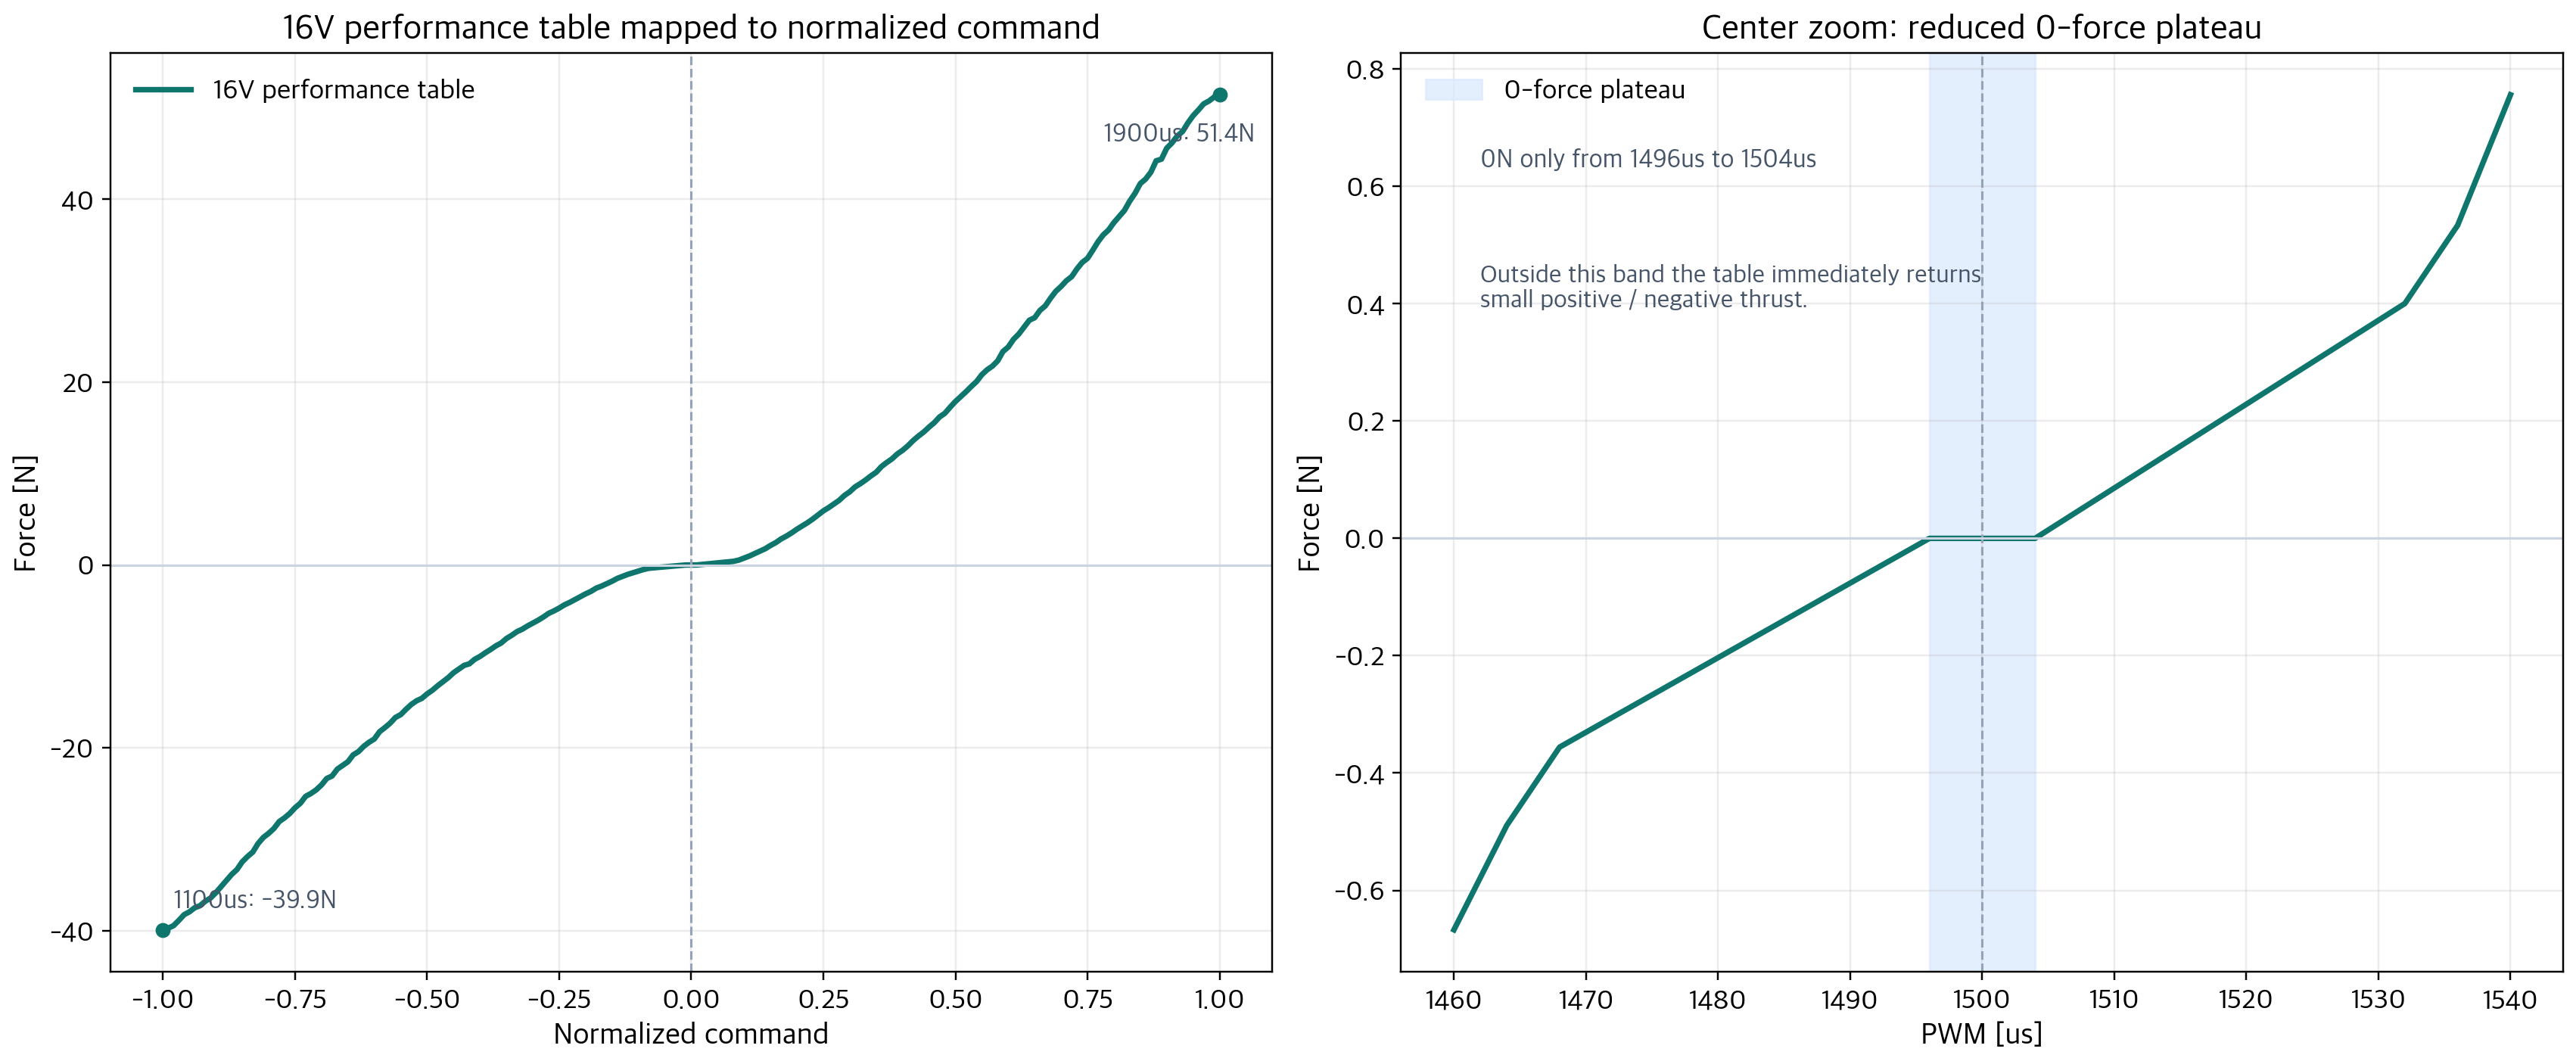
\includegraphics[width=0.96\linewidth]{figures_v22_latest/uuv_v22_latest_thruster_performance_curve.png}
  \caption{thruster performance reference graph. 좌측은 \code{thruster\_performance.json} 의 16V PWM-force 테이블이고, 우측은 그 테이블을 normalized command로 펼친 곡선과 current simple polynomial runtime model을 겹친 것이다. 즉 performance table은 reference 데이터이고, current default SITL path는 오른쪽의 simple polynomial model로 읽는 것이 맞다.}
\end{figure}

\begin{center}
\small
\begin{tabularx}{\linewidth}{>{\raggedright\arraybackslash}p{0.42\linewidth}Y}
\toprule
thrust 항목 & current 값 \\
\midrule
\code{deadzone} & 0.002 \\
\code{tau\_up}, \code{tau\_down} & 0.04\,s / 0.06\,s \\
\code{reverse\_asymmetry} & 0.7 \\
\code{gain\_scale\_all} & 2.9 \\
\code{command\_limit} & 1 \\
\code{forward\_poly} & $(0, 1.9, 4.8, 11.8)$ \\
\code{reverse\_poly} & $(0, 1.4, 3.5, 9.4)$ \\
\code{vertical\_thruster\_gain\_scale} & 1.45 \\
\code{yaw\_torque\_scale} & 1.5 \\
\bottomrule
\end{tabularx}
\end{center}

thrust 처리 순서는 다음 한 줄로 정리하면 충분하다.

\begin{quote}
normalized command $\rightarrow$ first-order lag $\rightarrow$ deadzone / saturation $\rightarrow$ forward-reverse polynomial force curve $\rightarrow$ per-axis gain $\rightarrow$ \code{data.ctrl} + extra yaw torque
\end{quote}

\section{중심부력 vs 4-point 부력 비교}

current는 기본적으로 4-point buoyancy를 사용한다. 비교를 위해 같은 current scene, 같은 current thrust model, 같은 runtime mass / inertia, 같은 scripted harness에서 \textbf{single-point center} 와 \textbf{current 4-point} 를 나란히 돌렸다.

\begin{figure}[H]
  \centering
  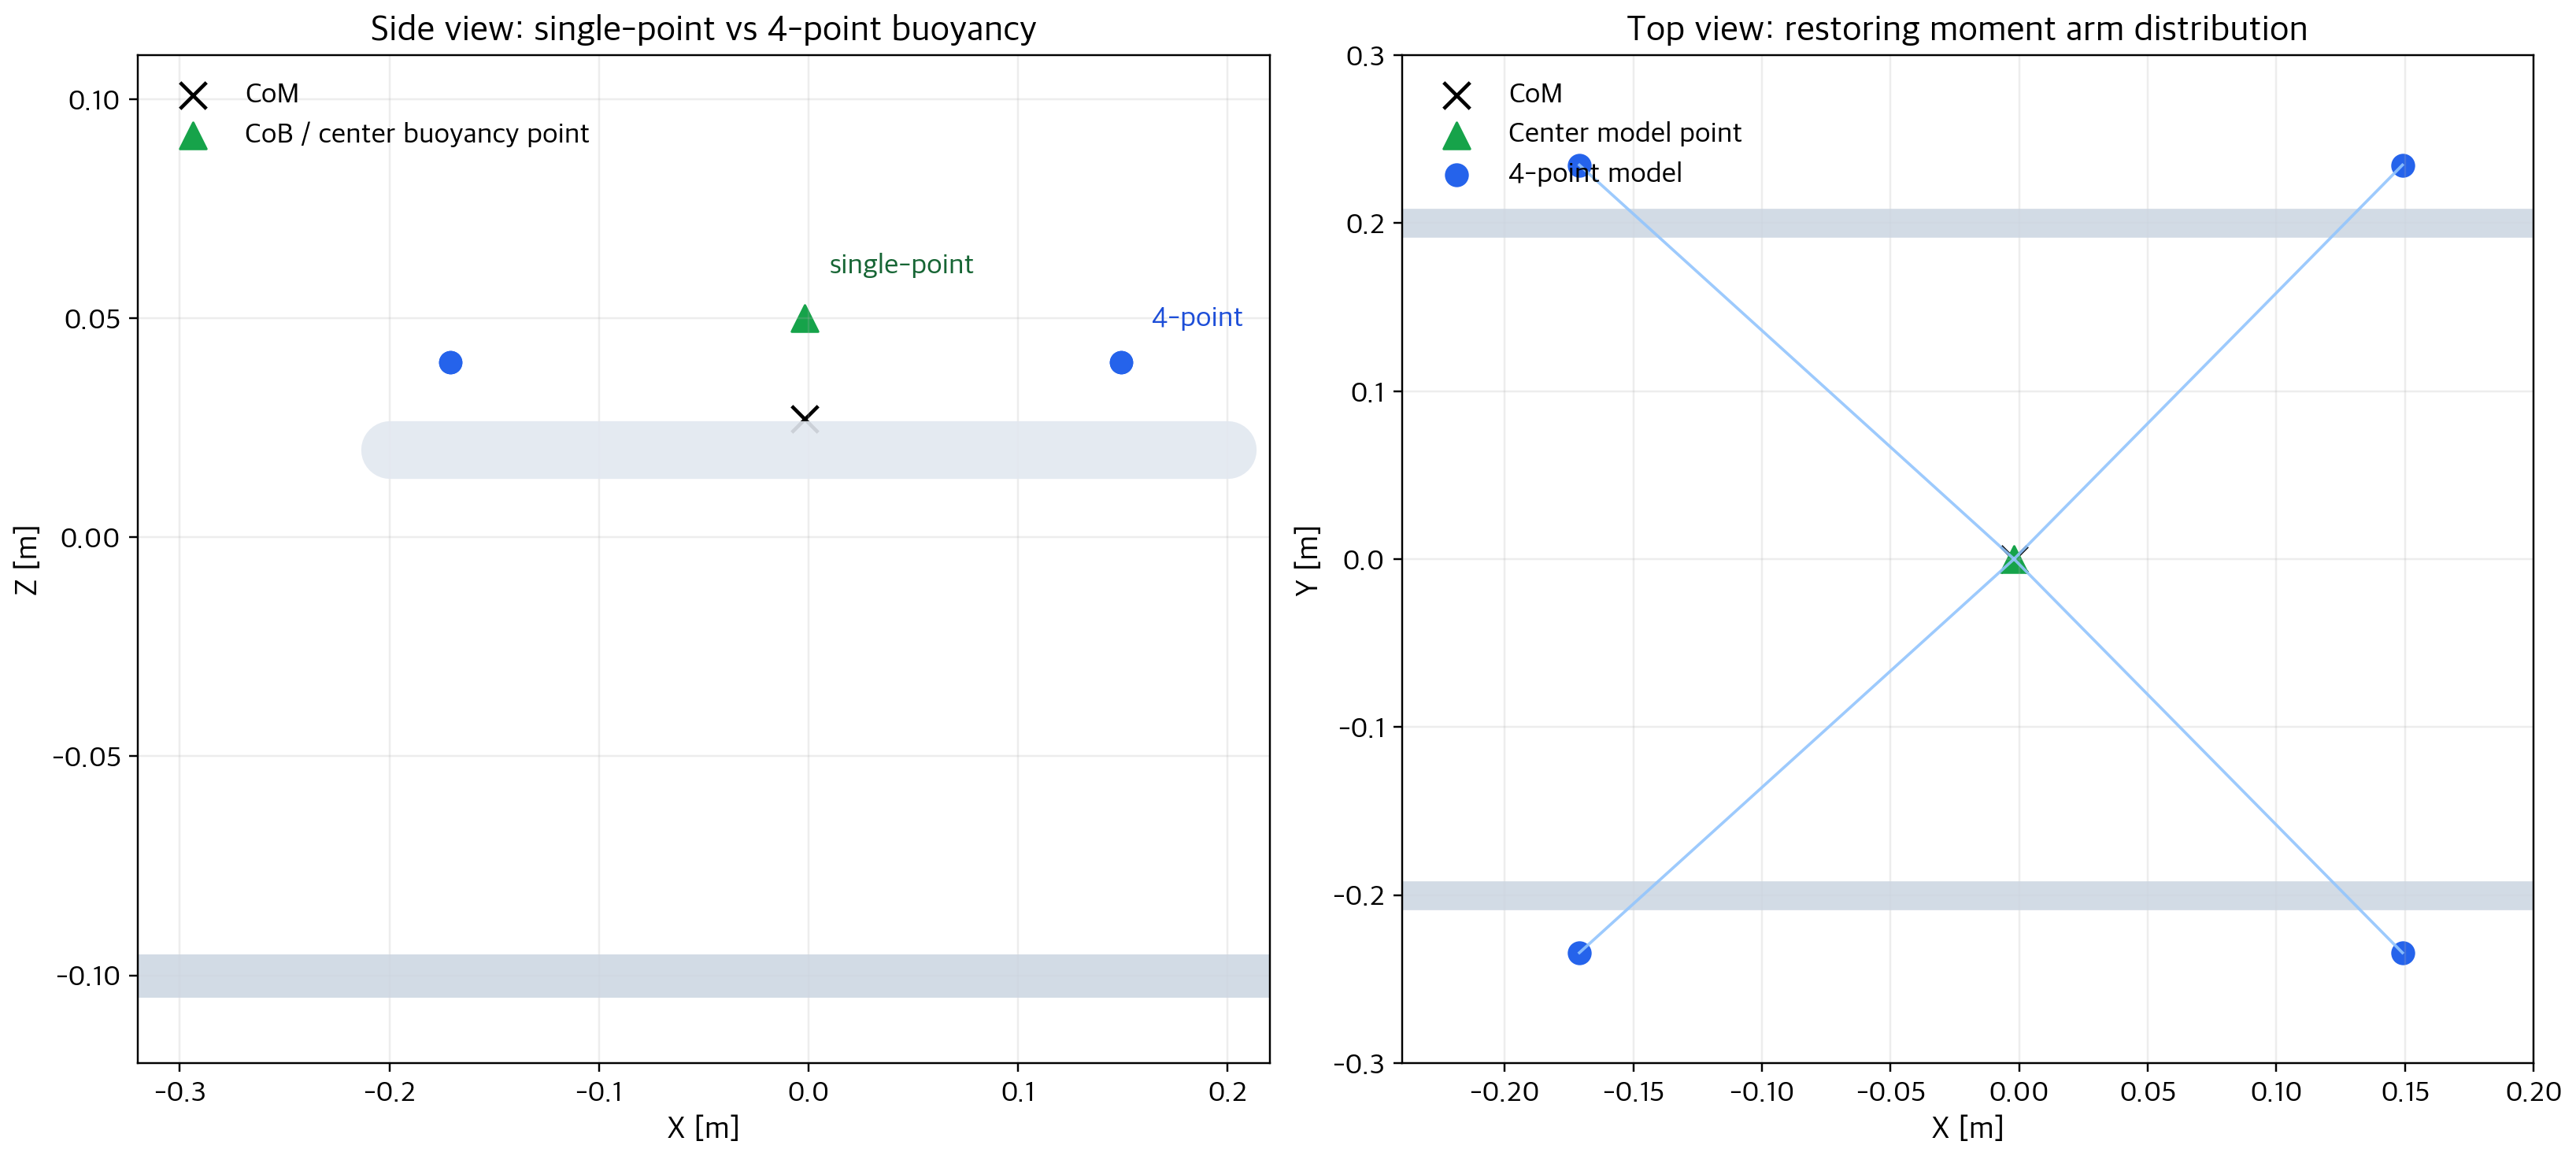
\includegraphics[width=0.96\linewidth]{figures_v22_latest/uuv_v22_latest_buoyancy_layout_compare.png}
  \caption{single-point center와 4-point buoyancy의 작용점 차이. center 모델은 총 buoyancy를 한 점에 모아서 적용하고, current 4-point는 같은 총 buoyancy를 네 점에 나눠 적용한다.}
\end{figure}

이번 비교에서 쓴 direct harness command는 forward 0.5, heave 0.023 이다. forward는 latest step의 nominal command를 그대로 사용했고, heave는 direct harness가 ArduSub RC/servo mapping을 건너뛰기 때문에 latest manual depth delta를 기준으로 4-point 모델이 맞는 수준으로 보정했다.

latest actual reference는 아래 네 값을 썼다.

\begin{itemize}[leftmargin=2em]
  \item forward peak surge: latest \code{stabilize\_forward\_step}
  \item forward peak pitch / roll: latest \code{stabilize\_forward\_step}
  \item heave depth delta: latest \code{manual\_heave\_step}
\end{itemize}

\begin{center}
\small
\begin{tabularx}{\linewidth}{>{\raggedright\arraybackslash}p{0.28\linewidth}YYY}
\toprule
항목 & single-point center & current 4-point & latest actual ref \\
\midrule
forward peak surge [m/s] & 0.497 & 0.644 & 0.557 \\
forward peak $|$pitch$|$ [deg] & 65.043 & 15.812 & 13.652 \\
forward peak $|$roll$|$ [deg] & 0.236 & 0.512 & 0.836 \\
heave depth delta [mm] & 3.67 & 40.33 & 42.34 \\
\bottomrule
\end{tabularx}
\end{center}

\begin{center}
\small
\begin{tabularx}{\linewidth}{>{\raggedright\arraybackslash}p{0.30\linewidth}YY}
\toprule
stability / similarity 지표 & single-point center & current 4-point \\
\midrule
attitude release RMS angle [deg] & 31.80 & 1.96 \\
attitude release settling time [s] & 5.998 & 0.554 \\
actual gap index [\%] & 137.61 & 18.72 \\
\bottomrule
\end{tabularx}
\end{center}

\begin{figure}[H]
  \centering
  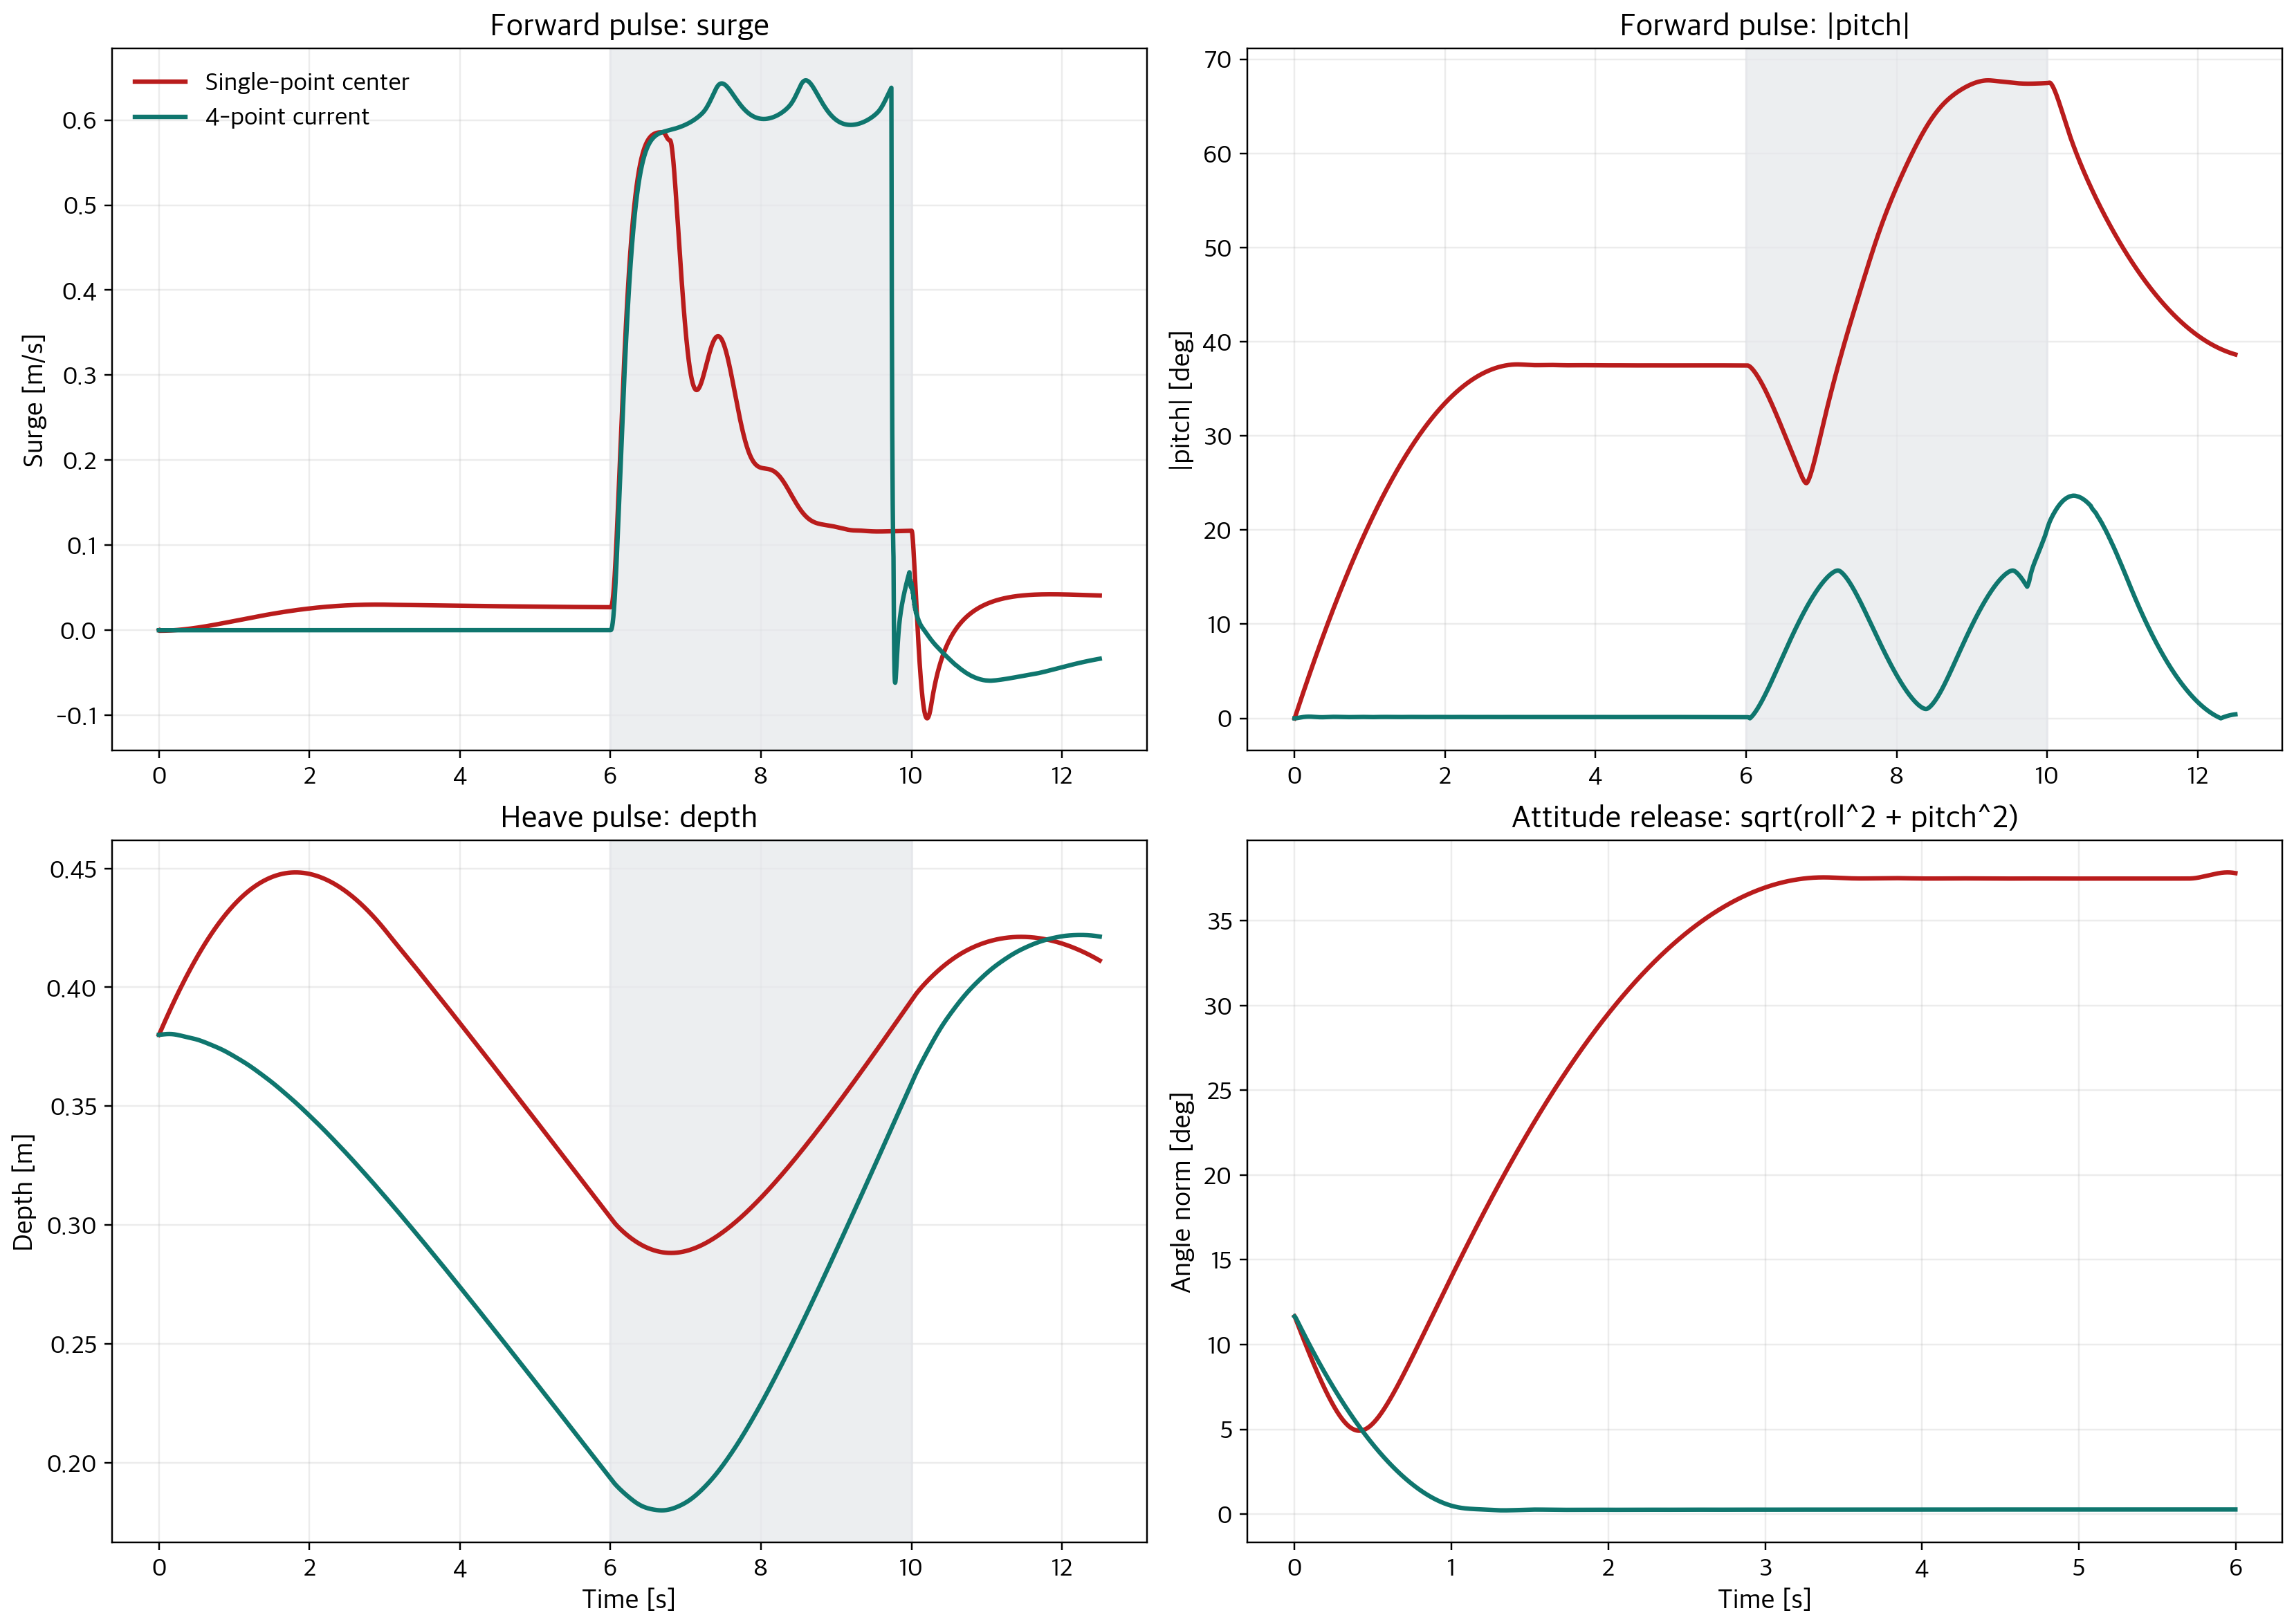
\includegraphics[width=0.98\linewidth]{figures_v22_latest/uuv_v22_latest_buoyancy_variant_responses.png}
  \caption{same current harness에서 center / 4-point buoyancy response 비교. 4-point는 forward pitch와 attitude release가 훨씬 빨리 수렴하고, heave에서도 latest actual reference와 같은 order의 depth delta를 만든다.}
\end{figure}

\begin{figure}[H]
  \centering
  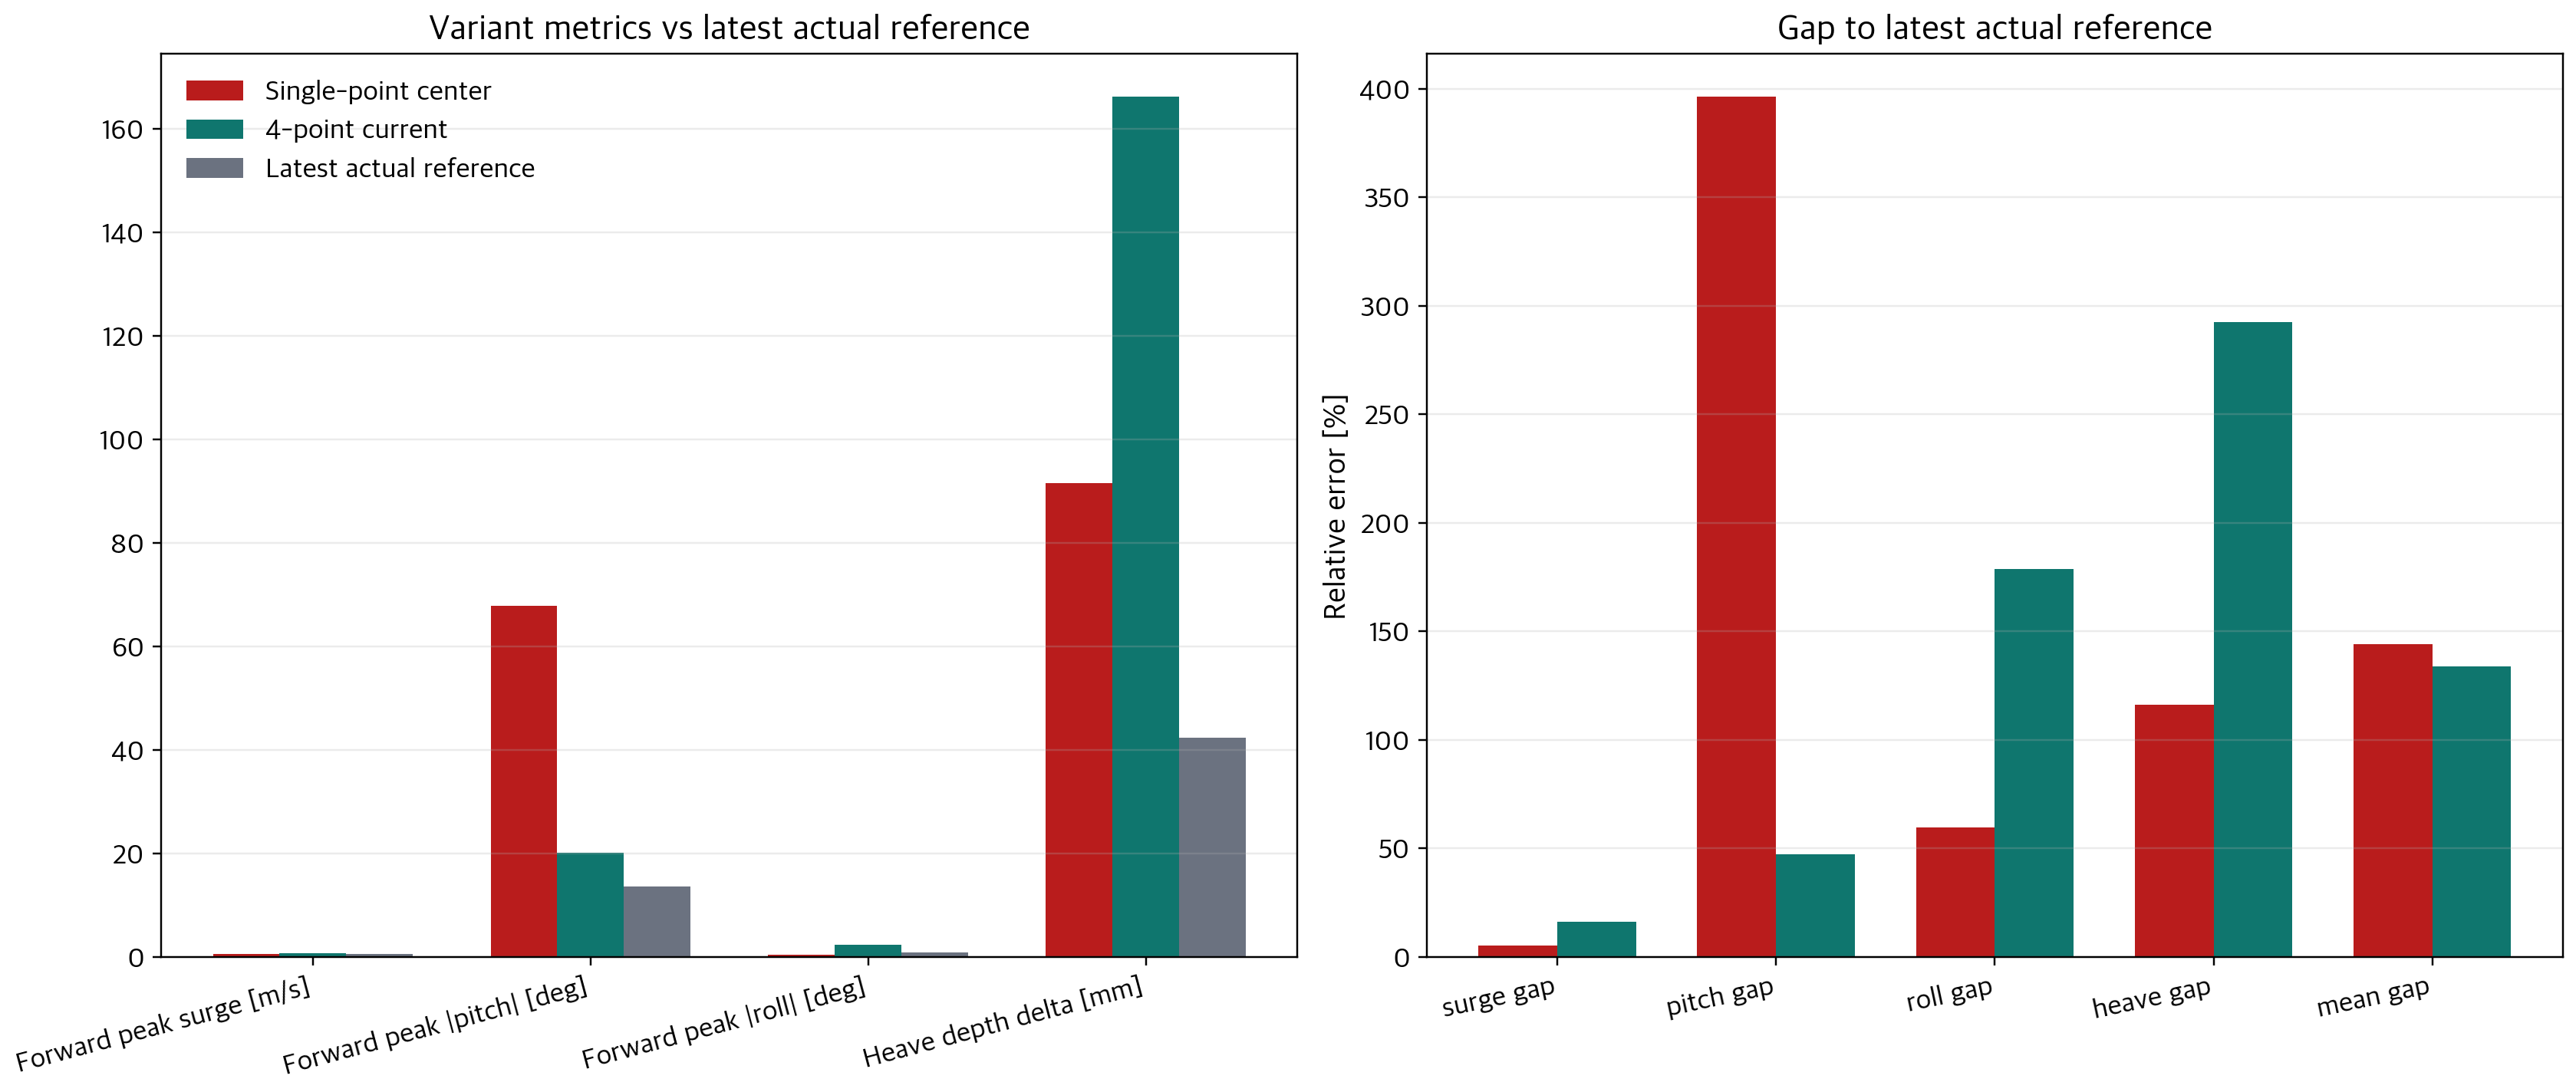
\includegraphics[width=0.98\linewidth]{figures_v22_latest/uuv_v22_latest_buoyancy_variant_metrics.png}
  \caption{center / 4-point / latest actual reference의 key metric 비교와 gap summary. current 4-point의 mean gap이 center보다 크게 낮다.}
\end{figure}

\section{latest current actual reference}

actual current latest bag만 따로 보면 평균 motion envelope는 아래와 같다.

\begin{center}
\small
\begin{tabularx}{\linewidth}{>{\raggedright\arraybackslash}p{0.36\linewidth}Y}
\toprule
current actual 평균값 & 값 \\
\midrule
평균 trajectory path length & 0.122\,m \\
평균 horizontal distance & 0.0273\,m \\
평균 max $|$pitch$|$ & 0.0885$^\circ$ \\
평균 max $|$roll$|$ & 0.0809$^\circ$ \\
\bottomrule
\end{tabularx}
\end{center}

\begin{center}
\small
\begin{tabularx}{\linewidth}{>{\raggedright\arraybackslash}p{0.18\linewidth}YYYY}
\toprule
모드 & path [m] & horizontal [m] & pitch [deg] & roll [deg] \\
\midrule
MANUAL & 0.170 & 0.012 & 0.175 & 0.229 \\
STABILIZE & 0.108 & 0.026 & 0.114 & 0.053 \\
ALT\_HOLD & 0.105 & 0.035 & 0.034 & 0.024 \\
POSHOLD & 0.105 & 0.037 & 0.031 & 0.018 \\
\bottomrule
\end{tabularx}
\end{center}

\begin{center}
\small
\begin{tabularx}{\linewidth}{>{\raggedright\arraybackslash}p{0.40\linewidth}YY}
\toprule
latest step summary 항목 & 값 & 해석 \\
\midrule
manual forward peak surge & 0.557\,m/s & current manual forward authority \\
stabilize forward peak surge & 0.557\,m/s & stabilize에서도 surge authority는 유지 \\
stabilize forward peak pitch & 13.65$^\circ$ & forward 입력 시 posture coupling \\
stabilize forward peak roll & 0.84$^\circ$ & roll coupling은 pitch보다 작음 \\
manual yaw peak rate & 0.790\,rad/s & yaw authority \\
manual heave depth delta & 42.34\,mm & latest manual heave response \\
alt-hold heave depth delta & 52.88\,mm & alt-hold heave response \\
\bottomrule
\end{tabularx}
\end{center}

\begin{figure}[H]
  \centering
  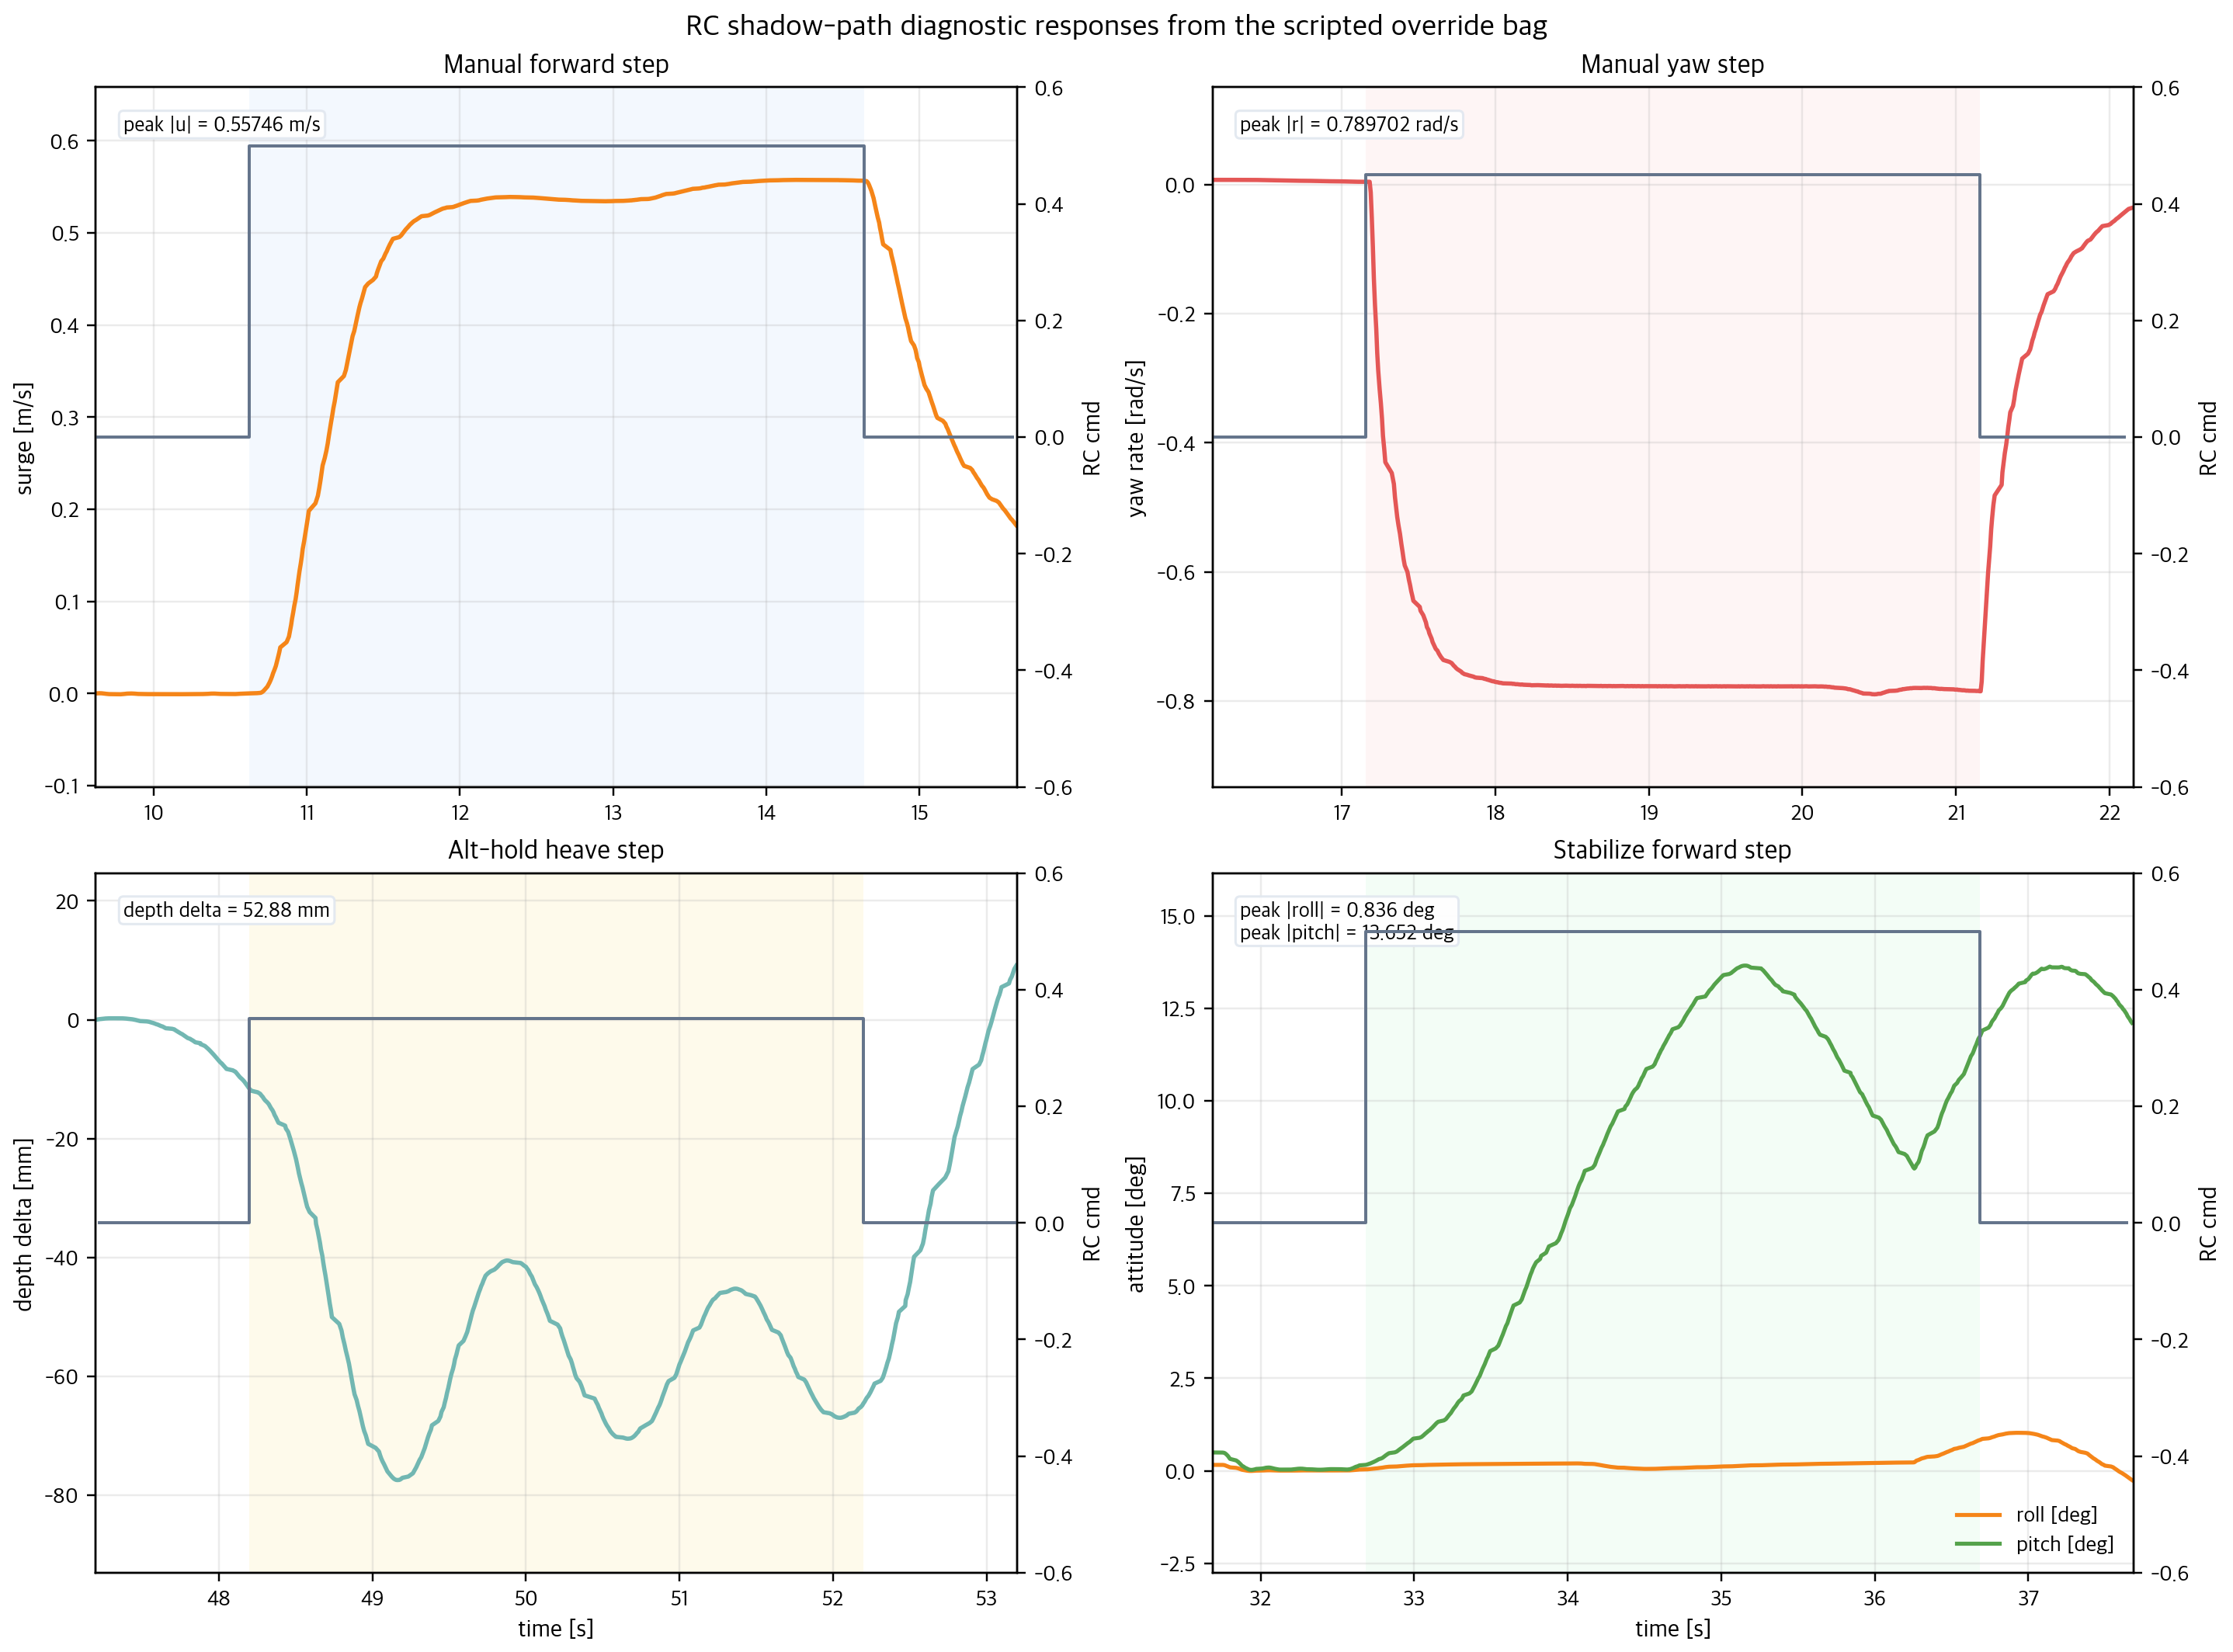
\includegraphics[width=0.98\linewidth]{figures_v22_latest/uuv_v22_latest_actual_step_responses.png}
  \caption{latest heavefix step bag 기반 current actual response. current 해석에서 직접 reference로 삼은 값들은 이 측정에서 왔다.}
\end{figure}

\begin{figure}[H]
  \centering
  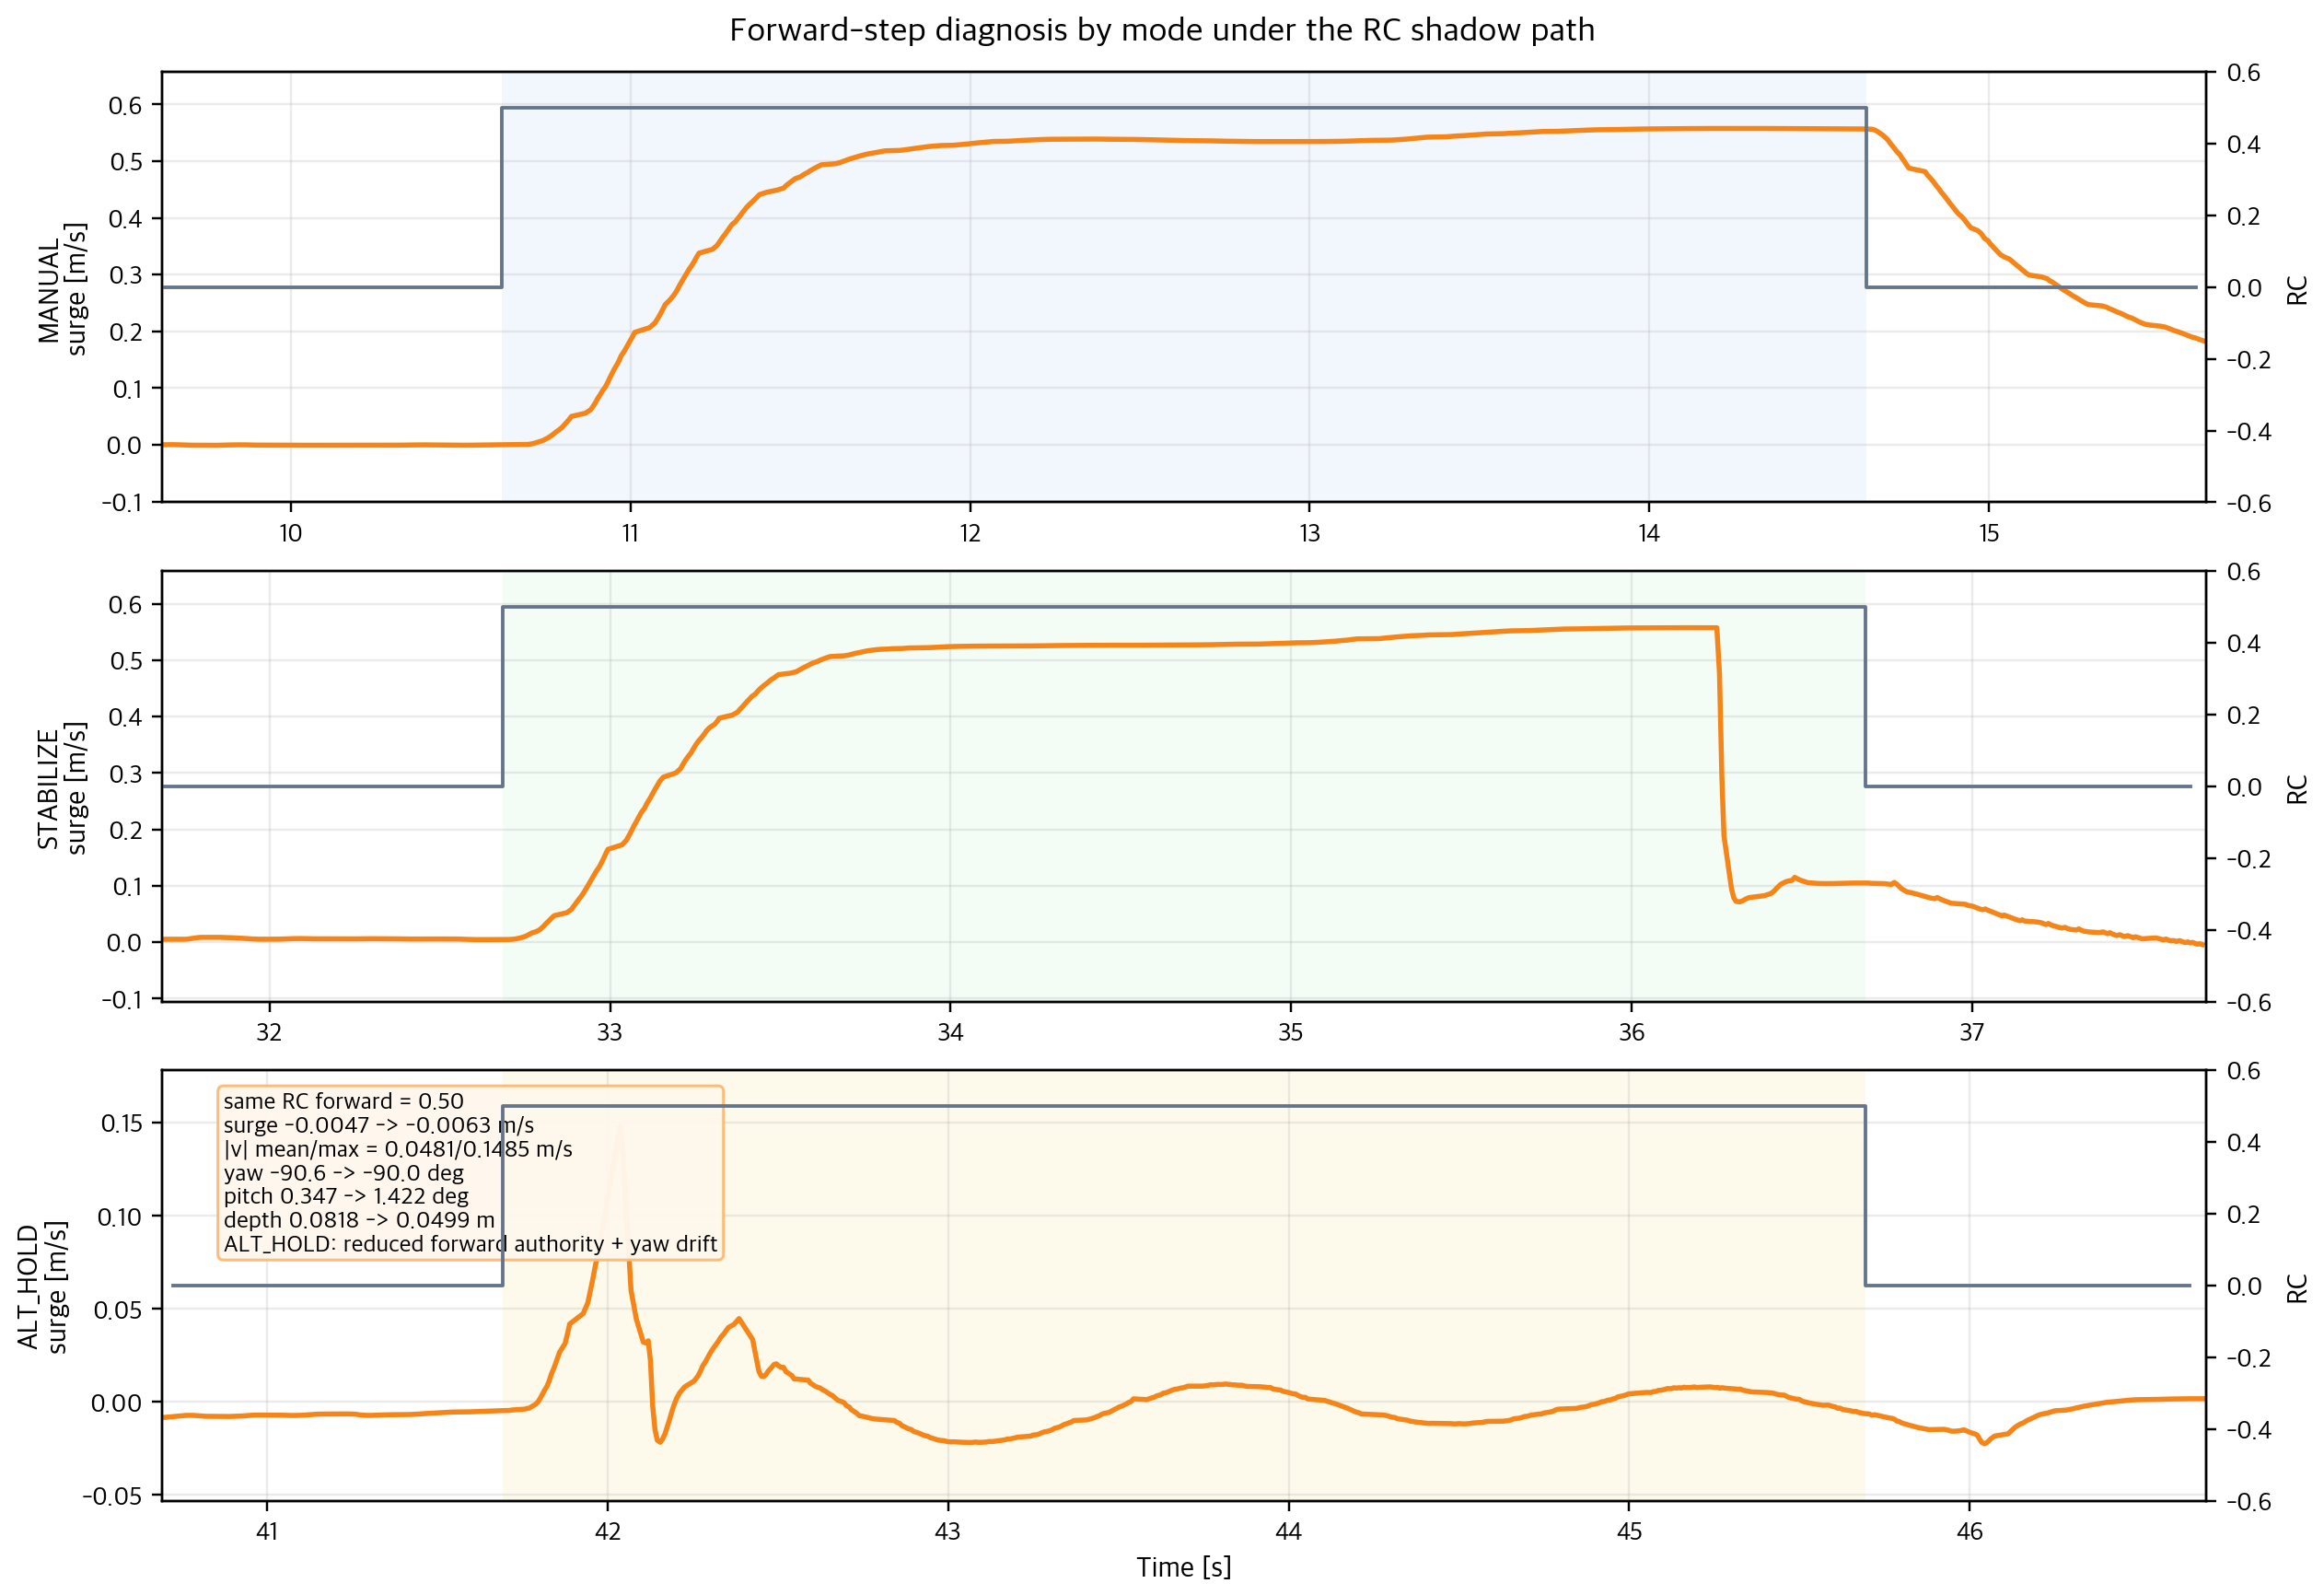
\includegraphics[width=0.96\linewidth]{figures_v22_latest/uuv_v22_latest_actual_mode_response.png}
  \caption{manual / stabilize / alt\_hold forward response 비교. current actual에서 mode별 response imbalance를 직접 확인할 수 있는 그림이다.}
\end{figure}

\section{정리}

current를 발표용으로 줄이면 아래 세 문장만 남기면 된다.

\begin{enumerate}[leftmargin=2em]
  \item current v2.2는 \textbf{MuJoCo ellipsoid fluid로 drag와 적분을 처리하고, Python runtime이 thrust model과 hydrostatics를 감싼 하이브리드 구조}다.
  \item thrust path는 simple polynomial model이고, hydrostatics는 current에서 \textbf{4-point buoyancy + restoring torque + runtime mass / inertia synthesis} 가 핵심이다.
  \item same current harness 기준으로 \textbf{4-point buoyancy가 single-point center보다 latest actual current reference에 훨씬 가깝고, release stability도 더 좋다}. 이것이 current 문서에서 4-point buoyancy를 따로 강조해야 하는 이유다.
\end{enumerate}

\end{document}
